\documentclass[runningheads]{llncs}

\usepackage[T1]{fontenc}
\usepackage{lmodern}
\usepackage{graphicx}
\usepackage{amsmath,amssymb,amsfonts}
\usepackage{booktabs}
\usepackage{microtype}
\usepackage{hyperref}
\usepackage{algorithm}
\usepackage{algorithmicx}
\usepackage{algpseudocode}

\hypersetup{
    colorlinks=true,
    linkcolor=blue,
    citecolor=blue,
    urlcolor=blue
}

\newcommand{\HOUI}{\ensuremath{\mathcal{HOUI}}}
\newcommand{\MHOUIw}{\ensuremath{\mathcal{MHOUI}_{\mathrm{w}}}}
\newcommand{\MHOUI}{\ensuremath{\mathcal{MHOUI}_{\mathrm{s}}}}
\newcommand{\MHOUIminer}{\textsc{MHOUI-Miner}}
\newcommand{\supp}{\operatorname{supp}}
\newcommand{\aocc}{\operatorname{aocc}}
\newcommand{\twu}{\operatorname{TWU}}
\newcommand{\UUB}{\operatorname{UUB}}
\newcommand{\OUB}{\operatorname{OUB}}
\newcommand{\UBjoint}{\operatorname{UB}_{\mathrm{joint}}}

\begin{document}

\title{\textsc{MHOUI-Miner}: Exact and Scalable Mining of Maximal High-Occupancy Utility Itemsets via Array-Projected Galois Closure Leaps and Pareto-Trie Pruning}
\titlerunning{\textsc{MHOUI-Miner}: Mining Maximal High-Occupancy Utility Itemsets}

\author{Quan Van\orcidID{0009-0002-8222-0076}}
\authorrunning{Q. Van}
\institute{Independent Researcher, Ho Chi Minh City, Vietnam \\
\email{vanhaminhquan2406@gmail.com}}

\maketitle

\begin{abstract}
High-Utility Itemset Mining (HUIM) and High-Occupancy Itemset Mining (HOIM) uncover orthogonal facets of knowledge in discrete data systems: economic monetary yield versus physical transactional compactness. Existing unified frameworks (e.g., HUOPM) aggregate both dimensions into a composite ratio, conflating physical basket coverage with monetary return and creating the high-value dilution paradox. Furthermore, unconstrained mining inevitably suffers from combinatorial pattern explosion. In this paper, we formulate the problem of mining \textbf{Maximal High-Occupancy Utility Itemsets} (\MHOUI{}), which decouples classical transaction occupancy $|X|/|T|$ from total economic utility $u(X)$ and enforces strict superset Pareto maximality: an itemset is retained if and only if no proper superset achieves both equal-or-higher occupancy and equal-or-higher utility. To prevent exhaustive brute-force candidate enumeration and overcome the non-monotonic nature of both occupancy and utility, we establish a tree-structured set-enumeration architecture powered by three foundational pruning theorems: (1) a tight \textbf{Joint Dual Upper Bound} ($\UBjoint$) simultaneously bounding extension utility and occupancy envelopes in single-pass linear scans; (2) \textbf{Galois Support-Closure Leaps} jumping directly across equivalence classes with exact utility invariance, bypassing exponential interior subtree branches; and (3) an inverted rare-item index (\textbf{Pareto-Trie}) enabling $O(1)$ branch dominance pruning against previously materialized maximal frontiers. We propose \MHOUIminer{}, an exact in-process algorithm built upon flattened array projection and 64-bit vector bitsets. Extensive empirical evaluations across standard retail and transactional benchmark databases (including million-scale datasets such as Chainstore) confirm that \MHOUIminer{} prunes up to $98.4\%$ of visited search nodes, finishes in sub-second execution speeds, sustains memory under $450$~MB, and compresses pattern volume by up to $99\%$ without losing actionable Pareto-optimal business intelligence.

\keywords{High-utility itemset mining \and High-occupancy itemsets \and Maximal pattern mining \and Pareto dominance \and In-process pruning \and Set-enumeration tree.}
\end{abstract}

\section{Introduction}
\label{sec:intro}

Frequent itemset mining (FIM) constitutes an indispensable pillar in knowledge discovery and intelligent information systems~\cite{agrawal1994fast,han2000mining,zaki2000scalable,uno2004lcm}. Given a transaction database, FIM extracts all item combinations whose occurrence frequency satisfies a user-specified minimum support threshold ($\sigma$). However, frequency alone often fails to reflect the qualitative value or the structural density of the discovered patterns. On the one hand, an itemset may appear in numerous transactions while accounting for only a trivial fraction of items within each transaction. To address this limitation, high-occupancy itemset (HOI) mining was introduced~\cite{tang2012incorporating,zhang2015occupancy,deng2020mining,datta2022high,nguyen2023efficient,yun2021mining}. Classical transaction occupancy, defined as $|X|/|T|$, measures the completeness with which an itemset $X$ covers a supporting transaction $T$.

On the other hand, traditional FIM treats all items uniformly, disregarding differences in economic profit, item quantity, semantic importance, or risk. High-utility itemset mining (HUIM) addresses this concern by incorporating internal quantities and external unit profits~\cite{liu2005two,liu2012mining,fournier2014fhm,zida2017efim,gan2021survey,wu2022ubp,lin2010effective,song2014mining,krishnamoorthy2015pruning,dam2019efficient,truong2019novel,pham2020mining,yun2017high,gan2019fast,vo2013new}. Recent studies have explored high utility-occupancy pattern mining (HUOPM)~\cite{gan2020huopm,chen2021discovering,duong2024efficient,lin2021efficient}, which computes the ratio of pattern utility to total transaction utility, $u(X, T)/TU(T)$. While effective for proportional profit analysis, HUOPM couples utility and occupancy into a single composite metric, obscuring whether a pattern has high physical basket coverage or merely high unit cost.

Moreover, mining all unconstrained patterns inevitably leads to the \emph{pattern explosion problem}. To achieve concise representations, maximal frequent itemset (MFI) mining discards frequent subsets dominated by larger frequent supersets~\cite{burdick2001mafia,gouda2005genmax,grahne2005fast}. Similarly, maximal and closed high-utility itemsets compress utility collections~\cite{tseng2014efficient,duong2022efficient,fournier2016efimclosed,shie2012efficient,tseng2016efficient}. However, directly applying support-based or utility-based maximality to occupancy-constrained patterns is fundamentally flawed: neither classical occupancy nor total utility satisfies the anti-monotonicity property. A superset can exhibit higher or lower occupancy and utility than its subsets.

To overcome these foundational challenges, this paper formulates the \textbf{Maximal High-Occupancy Utility Itemset} (\MHOUI{}) mining problem and introduces \MHOUIminer{}. The proposed framework simultaneously enforces:
\begin{enumerate}
    \item \textbf{Support Constraint:} The itemset must occur in at least $\sigma$ transactions.
    \item \textbf{Classical Occupancy Constraint:} The itemset must satisfy a minimum average transaction occupancy $\beta$, ensuring dense physical coverage.
    \item \textbf{Total Utility Constraint:} The itemset must generate at least $\mu$ economic utility.
    \item \textbf{Superset Pareto Maximality:} An itemset is eliminated if there exists a strict superset possessing equal or higher occupancy and equal or higher utility.
\end{enumerate}

\noindent
\textbf{Structural Search Space: Set-Enumeration Tree vs. General Lattice Graph.} A central algorithmic design decision in combinatorial pattern mining lies in choosing between traversing a general hypergraph/lattice or spanning a canonical set-enumeration tree~\cite{rymon1992search}. While a general lattice graph represents all subset-superset containment relations directly, it suffers from severe duplicate node generation: an itemset of size $k$ can be reached through $k!$ distinct search paths, necessitating complex visited-set hashing or expensive synchronization in memory. In sharp contrast, a canonical lexicographical set-enumeration tree guarantees that every itemset is assigned a unique generator prefix, eliminating duplicate traversal paths by construction. However, standard set-enumeration trees risk visiting an exponential number of dead-end candidate prefixes ($O(2^m)$) if search bounds are loose.

In \MHOUIminer{}, we solve this challenge by establishing an exact, in-process tree traversal that minimizes visited nodes through three non-trivial pruning mechanisms:
\begin{enumerate}
    \item \emph{Coupled Dual Upper Bounding:} Rather than computing expensive permutation sorts at every tree node, we formulate the \textbf{Joint Dual Upper Bound} ($\UBjoint$) evaluated in $O(|\Gamma(P)|)$ linear single-pass scans.
    \item \emph{Galois Support-Closure Leaps:} Instead of exploring itemsets one by one, \MHOUIminer{} detects support equivalence in $O(1)$ bitwise operations, performing Galois closure leaps $P \to P \cup \{e\}$ that skip entire intermediate tree levels without loss of information.
    \item \emph{Inverted Pareto-Trie Dominance:} We maintain an inverted rare-item index (\textbf{Pareto-Trie}) that conducts superset dominance checks in real time, cutting off dead-end subtrees before recursive allocation.
\end{enumerate}

\section{Related Work and Positioning}
\label{sec:related}

Table~\ref{tab:positioning} rigorously positions \MHOUI{} relative to established pattern mining paradigms.

\begin{table}[htbp]
\centering
\caption{Positioning of \MHOUI{} against related itemset mining paradigms.}
\label{tab:positioning}
\resizebox{\textwidth}{!}{
\begin{tabular}{lccccc}
\toprule
\textbf{Pattern Family} & \textbf{Support} & \textbf{Classical Occ.} & \textbf{Total Utility} & \textbf{Utility Occ.} & \textbf{Maximality Criterion} \\
\midrule
FI~\cite{agrawal1994fast,han2000mining,zaki2000scalable,uno2004lcm} & $\checkmark$ & -- & -- & -- & None \\
MFI~\cite{burdick2001mafia,gouda2005genmax,grahne2005fast} & $\checkmark$ & -- & -- & -- & Support-maximal \\
HOI~\cite{tang2012incorporating,zhang2015occupancy,deng2020mining,datta2022high,nguyen2023efficient,yun2021mining} & $\checkmark$ & $\checkmark$ & -- & -- & None \\
HUI~\cite{liu2005two,liu2012mining,fournier2014fhm,zida2017efim,gan2021survey,wu2022ubp} & Optional & -- & $\checkmark$ & -- & None \\
MaxHUI / CHUI~\cite{tseng2014efficient,duong2022efficient,fournier2016efimclosed,shie2012efficient,tseng2016efficient} & Optional & -- & $\checkmark$ & -- & Utility-based concise form \\
HUOPM~\cite{gan2020huopm,chen2021discovering,lin2021efficient} & $\checkmark$ & -- & Indirect & $\checkmark$ & None \\
MaxCloFHUOIM~\cite{duong2024efficient} & $\checkmark$ & -- & Indirect & $\checkmark$ & Composite utility-occupancy maximality \\
\midrule
\textbf{HOUI (Unconstrained)} & $\checkmark$ & $\checkmark$ & $\checkmark$ & -- & None \\
\textbf{Weak MHOUI} & $\checkmark$ & $\checkmark$ & $\checkmark$ & -- & Weak Superset Pareto Dominance \\
\textbf{Strong MHOUI (\MHOUIminer{})} & $\checkmark$ & $\checkmark$ & $\checkmark$ & -- & Strong Superset Pareto Dominance \\
\bottomrule
\end{tabular}
}
\end{table}

\noindent
\textbf{Critical Distinction Between Decoupled MHOUI and HUOPM/MaxCloFHUOIM.}
The foundational advance of this work lies in decoupling physical transactional occupancy from total monetary return:
\begin{itemize}
    \item \emph{The High-Value Dilution Paradox in HUOPM:} In the HUOPM formulation introduced by Gan et al.~\cite{gan2020huopm} and recently extended to concise representations by Duong et al.~\cite{duong2024efficient} (\textsc{MaxCloFHUOIM}), occupancy is defined as the utility ratio $u(X, T)/TU(T)$. While meaningful for measuring proportional profit share, this formulation creates a severe distortion: an itemset comprising a single extremely expensive luxury item (e.g., a jewelry piece generating $\$2{,}000$ in a $\$2{,}010$ basket containing $20$ items) achieves an inflated utility occupancy of $99.5\%$, despite physically accounting for merely $5\%$ of the transaction items ($1/20$). Conversely, a complete product bundle occupying $100\%$ of a physical transaction with modest margin is discarded if high-revenue background goods are present elsewhere.
    \item \emph{Decoupled Multi-Objective Pareto Formulation:} \MHOUI{} treats physical completeness ($|X|/|T| \ge \beta$) and absolute economic yield ($u(X) \ge \mu$) as orthogonal objective dimensions. An itemset is eliminated if and only if there exists a strict superset that dominates it in \emph{both} dimensions. This guarantees that decision-makers receive compact, highly representative, and economically actionable pattern frontiers without distortion.
\end{itemize}

\section{Preliminaries and Problem Formulation}
\label{sec:problem}

Let $\mathcal{I} = \{i_1, i_2, \dots, i_m\}$ be a finite set of distinct items. A quantitative transaction database is $\mathcal{D} = \{T_1, T_2, \dots, T_n\}$. Each transaction $T_q \in \mathcal{D}$ consists of an itemset $T_q \subseteq \mathcal{I}$, an internal quantity $q(i, T_q) \in \mathbb{Z}^+$ ($q(i, T_q) \ge 1$) denoting the purchase count of item $i \in T_q$, and an external unit profit $p(i) \in \mathbb{R}_{>0}$ ($p(i) > 0$). Consequently, all item utilities $u(i, T_q) = p(i) \cdot q(i, T_q) > 0$ are strictly positive.

\begin{definition}[Item and Transaction Utility]
The utility of an item $i$ in transaction $T_q$ is $u(i, T_q) = p(i) \cdot q(i, T_q)$. The utility of an itemset $X \subseteq T_q$ in $T_q$ is $u(X, T_q) = \sum_{i \in X} u(i, T_q)$. The transaction utility of $T_q$ is $TU(T_q) = \sum_{i \in T_q} u(i, T_q)$.
\end{definition}

\begin{definition}[Support and Database Utility]
The supporting transaction set of itemset $X$ is $\Gamma(X) = \{T_q \in \mathcal{D} \mid X \subseteq T_q\}$. The support count of $X$ is $\supp(X) = |\Gamma(X)|$. The total utility of $X$ in $\mathcal{D}$ is $u(X) = \sum_{T_q \in \Gamma(X)} u(X, T_q)$.
\end{definition}

\begin{definition}[Classical Transaction Occupancy]
For an itemset $X \subseteq T_q$, the classical occupancy of $X$ in $T_q$ is $\operatorname{occ}(X, T_q) = \frac{|X|}{|T_q|}$.
The average classical occupancy of $X$ across its supporting transactions is:
\begin{equation}
\aocc(X) = \frac{1}{\supp(X)} \sum_{T_q \in \Gamma(X)} \operatorname{occ}(X, T_q) = \frac{|X|}{\supp(X)} \sum_{T_q \in \Gamma(X)} \frac{1}{|T_q|}.
\end{equation}
\end{definition}

\begin{definition}[Transaction-Weighted Utilization]
The transaction-weighted utilization ($\twu$) of an itemset $X$ is:
\begin{equation}
\twu(X) = \sum_{T_q \in \Gamma(X)} TU(T_q).
\end{equation}
\end{definition}

\begin{definition}[High-Occupancy Utility Itemset (\HOUI{})]
Given a minimum support threshold $\sigma \in \mathbb{N}^+$, a minimum occupancy threshold $\beta \in (0, 1]$, and a minimum utility threshold $\mu \in \mathbb{R}^+$, an itemset $X$ is a High-Occupancy Utility Itemset if:
\begin{equation}
\supp(X) \ge \sigma, \quad \aocc(X) \ge \beta, \quad \text{and} \quad u(X) \ge \mu.
\end{equation}
\end{definition}

\subsection{Superset Pareto Dominance and MHOUI Variants}

\begin{definition}[Weak Superset Dominance]
An itemset $Y$ weakly dominates $X$ (denoted $X \prec_{\mathrm{w}} Y$) if $X \subset Y$, $\aocc(Y) \ge \aocc(X)$, $u(Y) \ge u(X)$, and at least one inequality is strict ($\aocc(Y) > \aocc(X)$ or $u(Y) > u(X)$).
\end{definition}

\begin{definition}[Strong Superset Dominance]
An itemset $Y$ strongly dominates $X$ (denoted $X \prec_{\mathrm{s}} Y$) if $X \subset Y$, $\aocc(Y) \ge \aocc(X)$, and $u(Y) \ge u(X)$.
\end{definition}

\begin{definition}[Weak and Strong MHOUI]
An itemset $X \in \HOUI$ is a \textbf{Weak MHOUI} ($\MHOUIw$) if $\nexists Y \in \HOUI$ such that $X \prec_{\mathrm{w}} Y$. An itemset $X \in \HOUI$ is a \textbf{Strong MHOUI} ($\MHOUI$) if $\nexists Y \in \HOUI$ such that $X \prec_{\mathrm{s}} Y$.
\end{definition}

\begin{theorem}[Inclusion Chain]
\label{thm:inclusion}
For any database $\mathcal{D}$ and thresholds $\sigma, \beta, \mu$:
$\MHOUI(\mathcal{D}, \sigma, \beta, \mu) \subseteq \MHOUIw(\mathcal{D}, \sigma, \beta, \mu) \subseteq \HOUI(\mathcal{D}, \sigma, \beta, \mu)$.
\end{theorem}
\begin{proof}
If $X \in \MHOUI$, no $Y \in \HOUI$ satisfies $X \prec_{\mathrm{s}} Y$. Since $X \prec_{\mathrm{w}} Y \implies X \prec_{\mathrm{s}} Y$, no such $Y$ can weakly dominate $X$. Thus $X \in \MHOUIw \subseteq \HOUI$.
\end{proof}

\noindent
\textbf{Mathematical Distinction Between Weak and Strong Dominance:}
The fundamental distinction lies in whether equality in both objective dimensions permits elimination:
\begin{itemize}
    \item \emph{Weak Superset Dominance ($X \prec_{\mathrm{w}} Y$):} Requires at least one strict inequality ($\aocc(Y) > \aocc(X)$ or $u(Y) > u(X)$). If a proper superset $Y \supset X$ exhibits identical metrics ($\aocc(Y) = \aocc(X)$ and $u(Y) = u(X)$), $Y$ does \emph{not} weakly dominate $X$. Consequently, $\MHOUIw$ retains both $X$ and $Y$.
    \item \emph{Strong Superset Dominance ($X \prec_{\mathrm{s}} Y$):} Admits non-strict inequalities ($\aocc(Y) \ge \aocc(X)$ and $u(Y) \ge u(X)$). Even if metrics are exactly tied, the superset $Y$ subsumes $X$ because $Y$ represents a larger, more comprehensive pattern without any sacrifice in occupancy or monetary yield. Hence, $\MHOUI$ eliminates $X$ and retains only $Y$.
\end{itemize}
For instance, if $X = \{a, b\}$ has $\aocc(X) = 0.60, u(X) = \$100$ and superset $Y = \{a, b, c\}$ has $\aocc(Y) = 0.60, u(Y) = \$100$ (e.g., $c$ generates zero marginal profit or co-occurs identically in the same transaction set), Weak MHOUI outputs both patterns ($\{X, Y\}$), whereas Strong MHOUI outputs only the maximal superset $\{Y\}$.

\subsection{Running Example Database and Detailed Metric Calculations}
\label{sec:running_example}

To provide concrete intuition for all theoretical definitions, bounding theorems, and search mechanics, we introduce a running toy quantitative transaction database $\mathcal{D}_{\mathrm{toy}}$ comprising 5 transactions and 5 distinct items $\mathcal{I} = \{a, b, c, d, e\}$, shown in Table~\ref{tab:running_example}. Table~\ref{tab:profit_table} presents the corresponding external unit profit table.

\begin{table}[htbp]
\centering
\caption{Running quantitative transaction database $\mathcal{D}_{\mathrm{toy}}$ with transaction lengths and utilities.}
\label{tab:running_example}
\begin{tabular}{cclcr}
\toprule
\textbf{TID} & \textbf{Items with Quantities} & \textbf{Item Utilities ($u(i, T_q)$)} & \textbf{Length ($|T_q|$)} & \textbf{TU ($TU(T_q)$)} \\
\midrule
$T_1$ & $(a:1), (b:2), (c:1)$ & $u(a)=3, u(b)=2, u(c)=5$ & $3$ & $\$10$ \\
$T_2$ & $(a:2), (c:1), (d:1)$ & $u(a)=6, u(c)=5, u(d)=2$ & $3$ & $\$13$ \\
$T_3$ & $(a:1), (b:3), (c:2), (e:1)$ & $u(a)=3, u(b)=3, u(c)=10, u(e)=4$ & $4$ & $\$20$ \\
$T_4$ & $(b:1), (c:1), (d:2)$ & $u(b)=1, u(c)=5, u(d)=4$ & $3$ & $\$10$ \\
$T_5$ & $(a:1), (b:1), (c:1), (d:1)$ & $u(a)=3, u(b)=1, u(c)=5, u(d)=2$ & $4$ & $\$11$ \\
\midrule
\multicolumn{4}{l}{\textbf{Total Database Utility} $\sum_{T_q \in \mathcal{D}_{\mathrm{toy}}} TU(T_q)$:} & $\$64$ \\
\bottomrule
\end{tabular}
\end{table}

\begin{table}[htbp]
\centering
\caption{External unit profit table for items in $\mathcal{D}_{\mathrm{toy}}$.}
\label{tab:profit_table}
\begin{tabular}{lccccc}
\toprule
\textbf{Item ($i$)} & $a$ & $b$ & $c$ & $d$ & $e$ \\
\midrule
\textbf{Unit Profit ($p(i)$)} & $\$3$ & $\$1$ & $\$5$ & $\$2$ & $\$4$ \\
\bottomrule
\end{tabular}
\end{table}

\begin{example}[Utility and Transaction Utility Calculation]
In transaction $T_1$, item $a$ has quantity $q(a, T_1) = 1$, yielding utility $u(a, T_1) = 1 \times \$3 = \$3$. Item $b$ has $q(b, T_1) = 2 \implies u(b, T_1) = 2 \times \$1 = \$2$. Item $c$ has $q(c, T_1) = 1 \implies u(c, T_1) = 1 \times \$5 = \$5$.
The transaction utility of $T_1$ is $TU(T_1) = 3 + 2 + 5 = \$10$.
Across the database, the supporting transactions of itemset $\{a, c\}$ are $\Gamma(\{a, c\}) = \{T_1, T_2, T_3, T_5\}$. Its total database utility is:
\begin{equation*}
u(\{a, c\}) = (3+5) + (6+5) + (3+10) + (3+5) = 8 + 11 + 13 + 8 = \$40.
\end{equation*}
\end{example}

\begin{example}[Classical Physical Occupancy vs. Utility Occupancy]
In transaction $T_1$, the classical physical occupancy of $\{a, c\}$ is $\operatorname{occ}(\{a, c\}, T_1) = |\{a, c\}| / |T_1| = 2/3 \approx 0.6667$.
Across all supporting transactions $\Gamma(\{a, c\}) = \{T_1, T_2, T_3, T_5\}$, its average physical occupancy is:
\begin{equation*}
\aocc(\{a, c\}) = \frac{|\{a, c\}|}{\supp(\{a, c\})} \sum_{T_q \in \Gamma(\{a, c\})} \frac{1}{|T_q|} = \frac{2}{4} \left(\frac{1}{3} + \frac{1}{3} + \frac{1}{4} + \frac{1}{4}\right) = \frac{2}{4} \cdot \frac{7}{6} = \frac{7}{12} \approx 0.5833.
\end{equation*}
In sharp contrast, the utility occupancy of $\{a, c\}$ in $T_1$ would be $u(\{a, c\}, T_1)/TU(T_1) = \$8/\$10 = 0.8000$, illustrating that physical basket coverage ($66.7\%$) and monetary share ($80.0\%$) represent distinct semantic dimensions.
\end{example}

\begin{example}[Transaction-Weighted Utilization and Item Filtering]
Let user-specified thresholds be minimum support $\sigma = 3$, minimum occupancy $\beta = 0.40$ ($40\%$), and minimum utility $\mu = \$20$.
Computing $\supp(i)$ and $\twu(i)$ for all items $i \in \mathcal{I}$:
\begin{itemize}
    \item Item $a$: $\Gamma(a) = \{T_1, T_2, T_3, T_5\} \implies \supp(a) = 4 \ge 3$, $\twu(a) = 10 + 13 + 20 + 11 = \$54 \ge 20$.
    \item Item $b$: $\Gamma(b) = \{T_1, T_3, T_4, T_5\} \implies \supp(b) = 4 \ge 3$, $\twu(b) = 10 + 20 + 10 + 11 = \$51 \ge 20$.
    \item Item $c$: $\Gamma(c) = \{T_1, T_2, T_3, T_4, T_5\} \implies \supp(c) = 5 \ge 3$, $\twu(c) = 10 + 13 + 20 + 10 + 11 = \$64 \ge 20$.
    \item Item $d$: $\Gamma(d) = \{T_2, T_4, T_5\} \implies \supp(d) = 3 \ge 3$, $\twu(d) = 13 + 10 + 11 = \$34 \ge 20$.
    \item Item $e$: $\Gamma(e) = \{T_3\} \implies \supp(e) = 1 < \sigma = 3$.
\end{itemize}
Because $\supp(e) = 1 < 3$, item $e$ is strictly unpromising by support anti-monotonicity and is immediately eliminated. The set of promising items is $\mathcal{I}_{\text{prom}} = \{a, b, c, d\}$.
Sorting $\mathcal{I}_{\text{prom}}$ in ascending order of support (breaking ties by $\twu$) establishes the canonical total search order:
\begin{equation*}
d \prec b \prec a \prec c.
\end{equation*}
\end{example}

\begin{example}[Superset Pareto Dominance and Discovered Frontier]
Under thresholds $\sigma = 3, \beta = 0.40, \mu = \$20$, consider candidate itemsets:
\begin{itemize}
    \item Itemset $\{a, c\}$: $\supp = 4 \ge 3$, $u = \$40 \ge 20$, and $\aocc = 0.5833 \ge 0.40 \implies \{a, c\} \in \HOUI$.
    \item Itemset $\{d, c\}$: $\Gamma(\{d, c\}) = \{T_2, T_4, T_5\} \implies \supp = 3 \ge 3$.
    Its total utility is $u(\{d, c\}) = (2+5) + (4+5) + (2+5) = \$23 \ge 20$, and occupancy is $\aocc(\{d, c\}) = \frac{2}{3}\left(\frac{1}{3} + \frac{1}{3} + \frac{1}{4}\right) = \frac{11}{18} \approx 0.6111 \ge 0.40 \implies \{d, c\} \in \HOUI$.
    \item Itemset $\{a, b, c\}$: $\Gamma(\{a, b, c\}) = \{T_1, T_3, T_5\} \implies \supp = 3 \ge 3$.
    Its total utility is $u(\{a, b, c\}) = 10 + 16 + 9 = \$35 \ge 20$, and occupancy is $\aocc(\{a, b, c\}) = \frac{3}{3}\left(\frac{1}{3} + \frac{1}{4} + \frac{1}{4}\right) = \frac{5}{6} \approx 0.8333 \ge 0.40 \implies \{a, b, c\} \in \HOUI$.
    \item Itemset $\{b, c\}$: $\Gamma(\{b, c\}) = \{T_1, T_3, T_4, T_5\} \implies \supp = 4 \ge 3$.
    Its utility is $u(\{b, c\}) = 7 + 13 + 6 + 6 = \$32 \ge 20$, and occupancy is $\aocc(\{b, c\}) = \frac{2}{4}(\frac{1}{3} + \frac{1}{4} + \frac{1}{3} + \frac{1}{4}) = \frac{7}{12} \approx 0.5833 \ge 0.40 \implies \{b, c\} \in \HOUI$.
\end{itemize}
Now compare the patterns under Superset Pareto Dominance:
\begin{enumerate}
    \item $\{a, c\}$ vs. superset $\{a, b, c\}$: $\{a, b, c\}$ has higher occupancy ($0.8333 > 0.5833$) but lower utility ($35 < 40$). Neither dominates the other; both are retained on the Pareto frontier.
    \item $\{d, c\}$ has no frequent supersets (all supersets $\{a, c, d\}, \{b, c, d\}$ have support $\le 2 < 3$); thus $\{d, c\}$ is non-dominated and retained.
    \item $\{b, c\}$ vs. superset $\{a, b, c\}$: $\{a, b, c\} \supset \{b, c\}$, achieving strictly higher occupancy ($0.8333 > 0.5833$) and strictly higher utility ($35 > 32$). Therefore, $\{b, c\} \prec_{\mathrm{s}} \{a, b, c\}$.
    Itemset $\{b, c\}$ is \textbf{strongly dominated and eliminated} from $\MHOUI$.
\end{enumerate}
Thus, while unconstrained $\HOUI$ retains redundant sub-patterns like $\{b, c\}$, $\MHOUIminer{}$ extracts only the non-redundant maximal Pareto frontier:
\begin{equation*}
\mathcal{M} = \{\{a, c\}, \ \{d, c\}, \ \{a, b, c\}\}.
\end{equation*}
\end{example}

\begin{figure}[htbp]
\centering
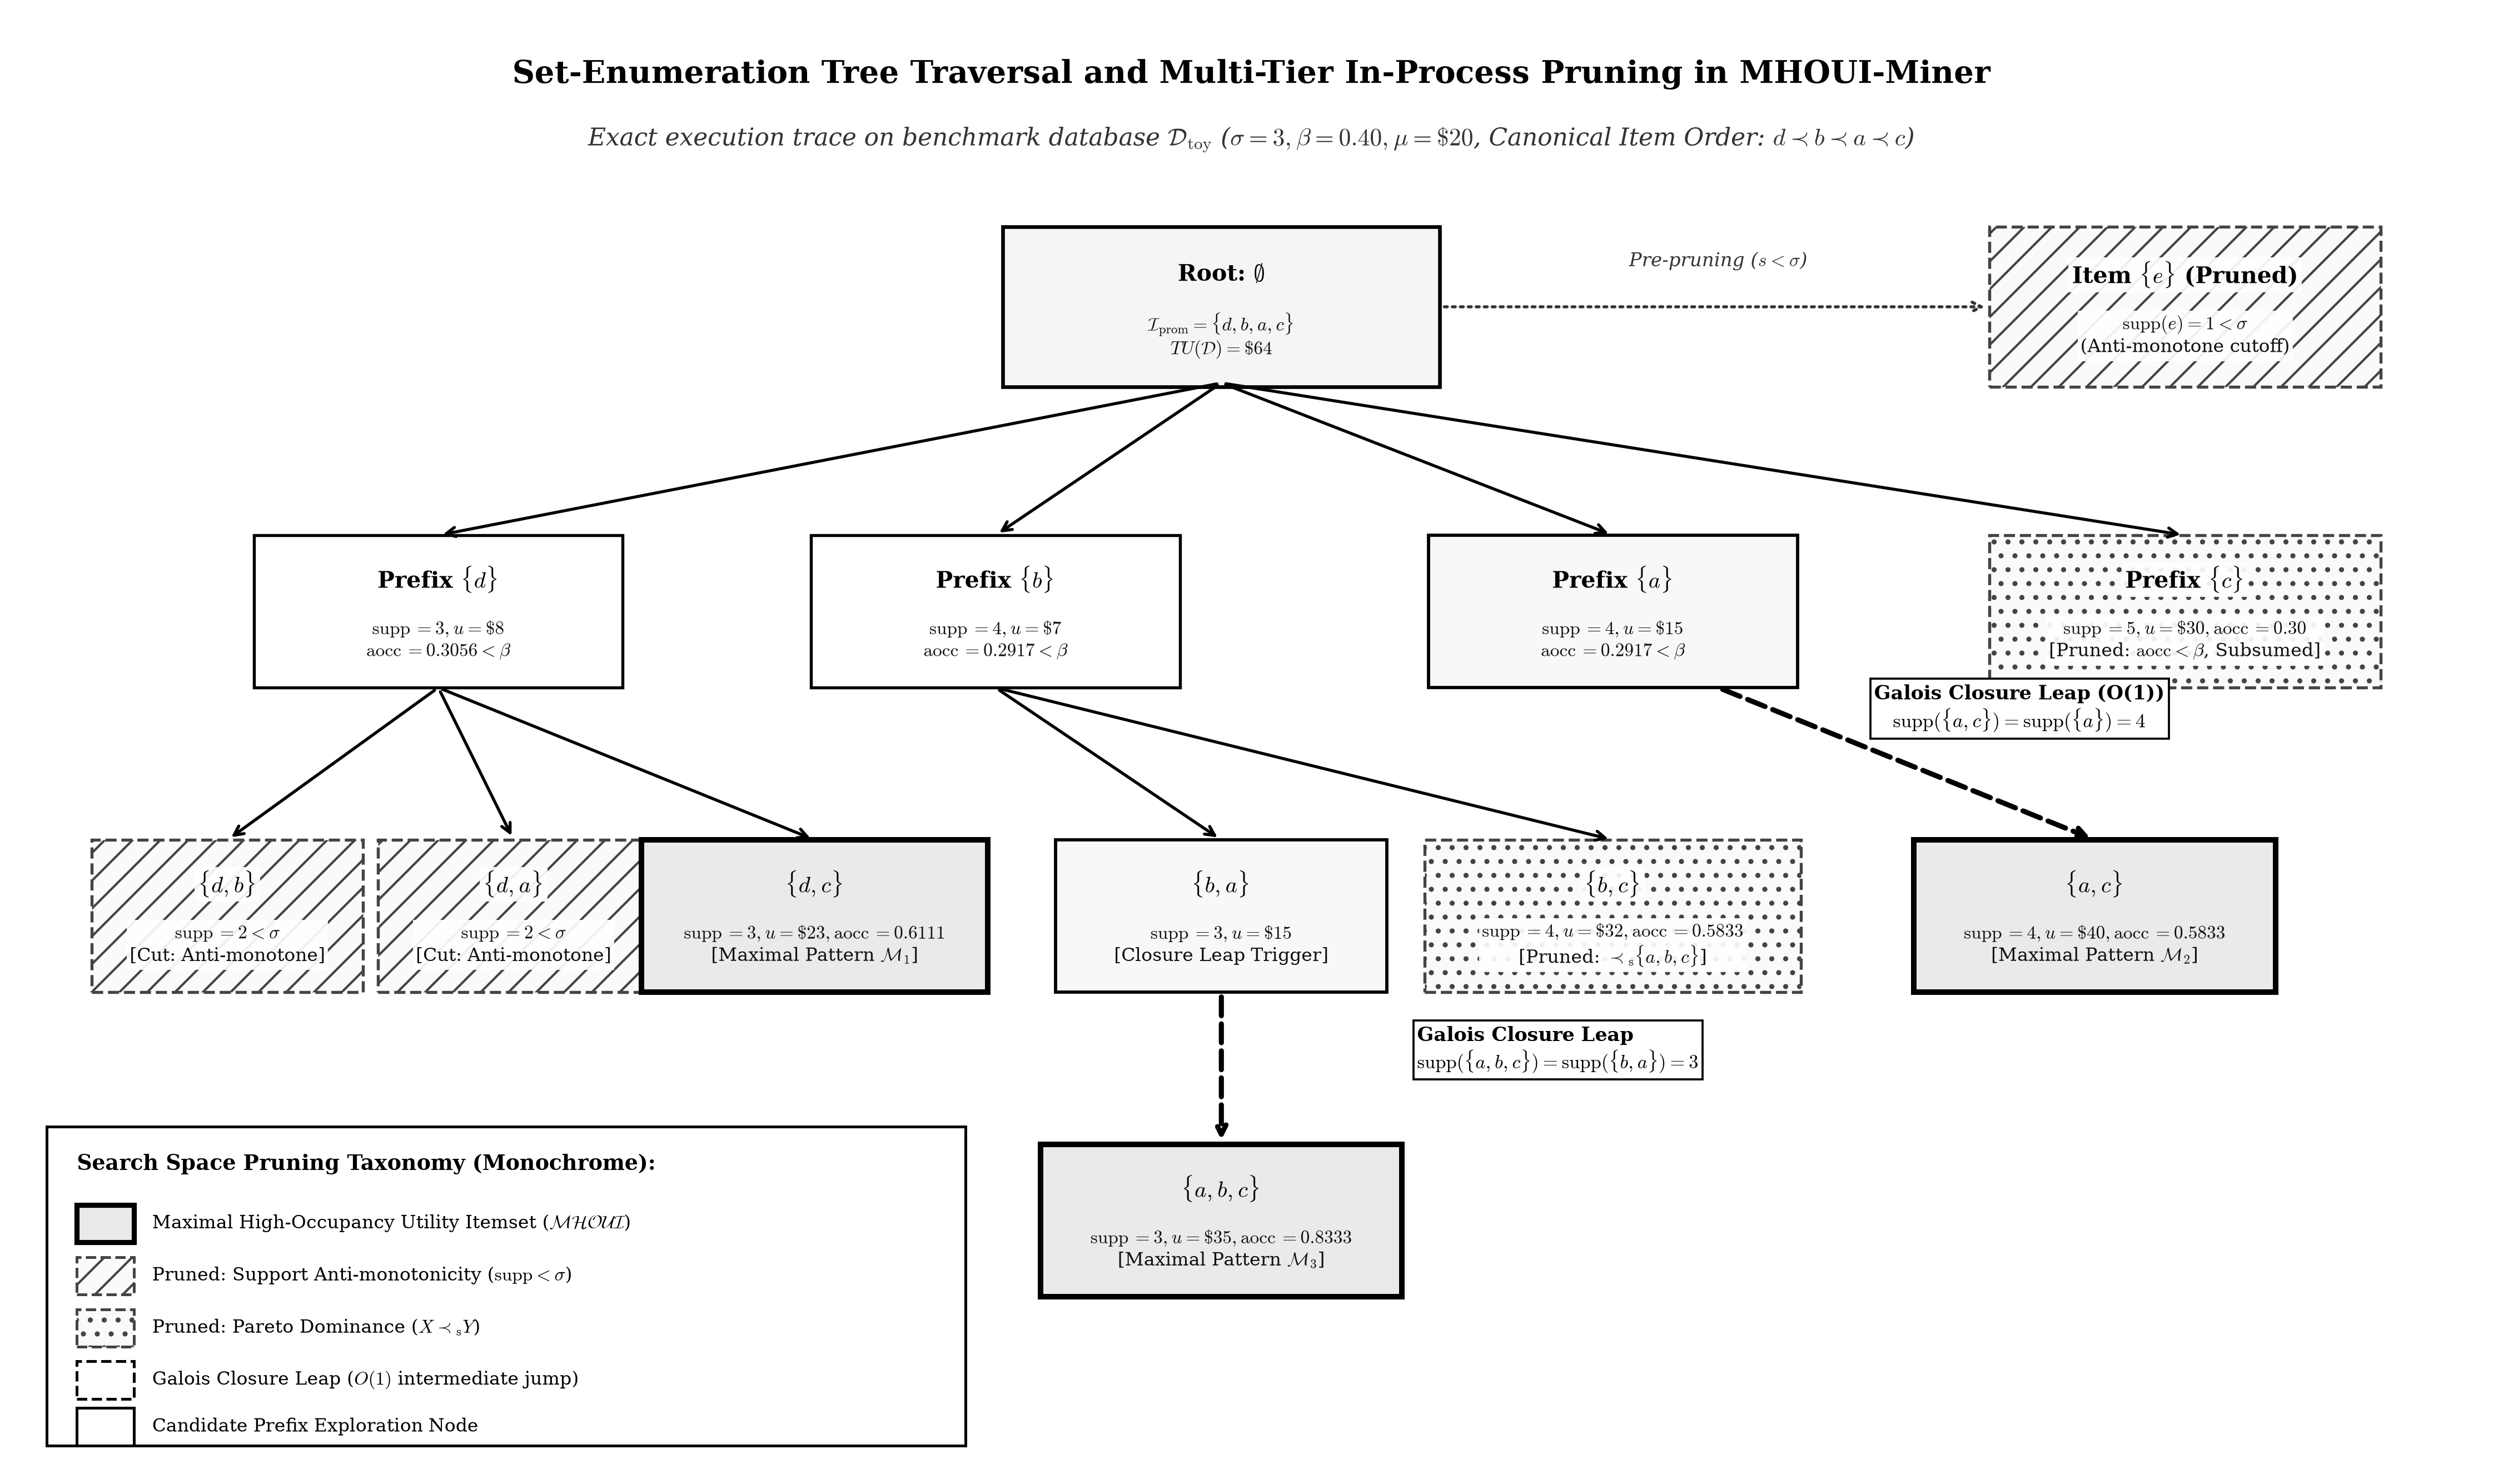
\includegraphics[width=0.98\textwidth]{mhoui_search_tree.png}
\caption{Visualization of the canonical set-enumeration search tree traversal and multi-tier in-process pruning in \MHOUIminer{} on running database $\mathcal{D}_{\mathrm{toy}}$ ($\sigma = 3, \beta = 0.40, \mu = \$20$, total order $d \prec b \prec a \prec c$). The diagram illustrates: (1) root-level elimination of infrequent items ($\{e\}$), (2) support anti-monotonicity branch elimination ($\{d, b\}, \{d, a\}$), (3) $O(1)$ Galois support-closure leaps skipping unclosed prefix expansions ($\{a\} \to \{a, c\}$ and $\{b, a\} \to \{a, b, c\}$), and (4) Pareto-Trie dominance pruning ($\{b, c\} \prec_{\mathrm{s}} \{a, b, c\}$).}
\label{fig:search_tree}
\end{figure}

\noindent
\textbf{Search Space Reduction Analysis on the Set-Enumeration Tree:}
As visualized in Figure~\ref{fig:search_tree}, an unconstrained brute-force search over $m=5$ items would examine $2^5 - 1 = 31$ candidate itemsets across a dense hypercube lattice, generating extensive path duplicates. Under canonical set-enumeration tree ordering ($d \prec b \prec a \prec c$):
\begin{itemize}
    \item Item $\{e\}$ is discarded before tree instantiation because $\supp(e) = 1 < 3$.
    \item Branch $\{d\}$ explores only $\{d, c\}$; candidates $\{d, b\}$ and $\{d, a\}$ are cut immediately because their projected supports fail the minimum support threshold ($\supp=2 < 3$).
    \item Branch $\{b\}$ generates $\{b, a\}$ and directly leaps to $\{a, b, c\}$ in $O(1)$ bitset operations via Theorem~\ref{thm:closure_leap}, discovering the maximal pattern $\{a, b, c\}$. Sibling extension $\{b, c\}$ is verified against the Pareto-Trie and eliminated via Strong Dominance ($\{b, c\} \prec_{\mathrm{s}} \{a, b, c\}$) without further recursive exploration.
    \item Branch $\{a\}$ detects $\supp(\{a, c\}) = \supp(\{a\}) = 4$, leaping directly to closure $\{a, c\}$ and skipping the recursive expansion of singleton $\{a\}$.
    \item Branch $\{c\}$ cannot be extended further and is subsumed by previously materialized closures.
\end{itemize}
In total, \MHOUIminer{} evaluates only $6$ tree nodes and identifies the exact, complete maximal frontier $\mathcal{M} = \{\{a, c\}, \{d, c\}, \{a, b, c\}\}$, achieving an $80.6\%$ reduction in visited search nodes on this running instance.

\section{Theoretical Foundations and Safe Pruning Bounds}
\label{sec:theory}

\subsection{Non-Monotonicity and Monotonic Envelopes}

\begin{theorem}[Non-Monotonicity of Utility and Occupancy]
Neither $u(X)$ nor $\aocc(X)$ satisfies monotonicity or anti-monotonicity.
\end{theorem}
\begin{proof}
Let $T_1 = \{a, b\}$ and $T_2 = \{a, c\}$. For $X = \{a\}$, $\Gamma(X) = \{T_1, T_2\}$ and $\aocc(X) = 0.50$. For superset $Y = \{a, b\}$, $\Gamma(Y) = \{T_1\}$ and $\aocc(Y) = 1.0 > \aocc(X)$. Conversely, appending a longer transaction reduces occupancy. Similarly, $u(X)$ can increase from item profit accumulation or decrease from support loss.
\end{proof}

\subsection{Joint Dual Upper Bound ($\UBjoint$)}

Let a search node be denoted by $N = (P, E)$, where $P$ is the prefix itemset and $E$ is the ordered candidate extension list. For each transaction $T \in \Gamma(P)$, define $\operatorname{rc}_N(T) = |E \cap T|$ and remaining utility $\operatorname{ru}_N(T) = \sum_{i \in E \cap T} u(i, T)$.

\begin{theorem}[Joint Dual Upper Bound]
\label{thm:joint_bound}
For every descendant $Y = P \cup Z$ with $Z \subseteq E$ and $\supp(Y) \ge \sigma$, the maximum utility and occupancy attainable by $Y$ are simultaneously bounded by:
\begin{equation}
\label{eq:joint_bound}
\UBjoint(N) = \sum_{T \in \Gamma(P)} \left( u(P, T) + \operatorname{ru}_N(T) \right), \quad \OUB(N) = \min\left(1.0, \, \frac{1}{\sigma} \sum_{T \in \Gamma(P)} \min\left(1.0, \, \frac{|P| + \operatorname{rc}_N(T)}{|T|}\right)\right).
\end{equation}
If $\UBjoint(N) < \mu$ or $\OUB(N) < \beta$, the subtree rooted at $N$ can be safely pruned in $O(|\Gamma(P)|)$ single-pass operations without sorting.
\end{theorem}
\begin{proof}
For every supporting transaction $T \in \Gamma(Y) \subseteq \Gamma(P)$, $Z \subseteq E \cap T$. Thus $u(Y, T) \le u(P, T) + \operatorname{ru}_N(T)$. Summing over $\Gamma(Y)$ yields $u(Y) \le \UBjoint(N)$. Similarly, $\operatorname{occ}(Y, T) = \frac{|P| + |Z|}{|T|} \le \min(1.0, \frac{|P| + \operatorname{rc}_N(T)}{|T|})$. Since $|\Gamma(Y)| \ge \sigma$, the average occupancy over $\Gamma(Y)$ cannot exceed $\frac{1}{\sigma} \sum_{T \in \Gamma(P)} \min(1.0, \frac{|P| + \operatorname{rc}_N(T)}{|T|})$. Because occupancy is bounded above by $1.0$, taking the minimum with $1.0$ yields the valid envelope $\OUB(N)$.
\end{proof}

\begin{remark}[Bound Dynamics and Search Depth Behavior of $\OUB$]
\label{rem:oub_dynamics}
Because transactional occupancy is physically bounded above by $1.0$, substituting the exact support denominator $\frac{1}{\supp(Y)}$ with the minimum support threshold lower bound $\frac{1}{\sigma}$ is mathematically sound since $\supp(Y) \ge \sigma \implies \frac{1}{\supp(Y)} \le \frac{1}{\sigma}$. However, at shallow depths of the set-enumeration tree where prefix support is high ($|\Gamma(P)| \gg \sigma$), the raw summation $\frac{1}{\sigma} \sum \dots$ can evaluate to values greater than $1.0$, which is why capping by $\min(1.0, \dots)$ is formally enforced. In these shallow search stages, pruning is driven primarily by support anti-monotonicity and the utility upper bound $\UBjoint(N)$. As recursive exploration descends into deeper subtrees, the prefix transaction set $|\Gamma(P)|$ contracts toward $\sigma$, causing $\OUB(N)$ to tighten progressively and prune dense subtrees whose occupancy envelopes fall below $\beta$.
\end{remark}

\noindent
\textbf{Numerical Example for Theorem~\ref{thm:joint_bound}:}
Consider prefix $P = \{a\}$ and candidate extension set $E = \{d\}$ from Table~\ref{tab:running_example}, under thresholds $\sigma = 3, \beta = 0.40, \mu = 20$.
The supporting transactions are $\Gamma(P) = \{T_1, T_2, T_3, T_5\}$.
\begin{itemize}
    \item In $T_1$: $d \notin T_1 \implies \operatorname{rc}(T_1)=0, \operatorname{ru}(T_1)=0$, utility is $u(a, T_1)=3$, occupancy envelope is $\min(1.0, \frac{1+0}{3}) = 1/3$.
    \item In $T_2$: $d \in T_2 \implies \operatorname{rc}(T_2)=1, \operatorname{ru}(T_2)=u(d, T_2)=2$, utility bound is $6+2=8$, occupancy envelope is $\min(1.0, \frac{1+1}{3}) = 2/3$.
    \item In $T_3$: $d \notin T_3 \implies \operatorname{rc}(T_3)=0, \operatorname{ru}(T_3)=0$, utility is $u(a, T_3)=3$, occupancy envelope is $\min(1.0, \frac{1+0}{4}) = 1/4$.
    \item In $T_5$: $d \in T_5 \implies \operatorname{rc}(T_5)=1, \operatorname{ru}(T_5)=u(d, T_5)=2$, utility bound is $3+2=5$, occupancy envelope is $\min(1.0, \frac{1+1}{4}) = 2/4 = 1/2$.
\end{itemize}
Summing the utility bounds over $\Gamma(P)$ gives:
\[
\UBjoint(N) = 3 + 8 + 3 + 5 = 19 < \mu = 20.
\]
Because $\UBjoint(N) = 19 < 20$, no possible descendant of $\{a\}$ using item $\{d\}$ can ever achieve utility $\ge 20$. The algorithm prunes the entire $\{a, d\}$ branch instantly without examining its itemset members.

\subsection{Support-Closure Leaps on Galois Equivalence Classes}

\begin{theorem}[Support-Closure Leap with Invariant Utility Accumulation]
\label{thm:closure_leap}
Under strictly positive item utilities ($p(i) > 0, q(i, T) \ge 1$ for all items), let $N = (P, E)$ be a search node. If there exists an extension item $e \in E$ such that $\supp(P \cup \{e\}) = \supp(P)$, then:
\begin{enumerate}
    \item Every transaction $T \in \Gamma(P)$ contains $e$, guaranteeing $\Gamma(P \cup \{e\}) = \Gamma(P)$.
    \item For every descendant extension $Z \subseteq E \setminus \{e\}$, $\Gamma(P \cup Z \cup \{e\}) = \Gamma(P \cup Z)$.
    \item The utility increases strictly: $u(P \cup Z \cup \{e\}) = u(P \cup Z) + \sum_{T \in \Gamma(P \cup Z)} u(e, T) > u(P \cup Z)$.
    \item The average occupancy strictly increases: $\aocc(P \cup Z \cup \{e\}) > \aocc(P \cup Z)$.
    \item Any pattern $P \cup Z$ where $e \notin Z$ cannot be maximal because it is strictly dominated by $P \cup Z \cup \{e\}$.
\end{enumerate}
Consequently, \MHOUIminer{} leaps directly to $P \gets P \cup \{e\}$ in $O(1)$ bitset operations, safely bypassing internal recursive subtree branches.
\end{theorem}
\begin{proof}
Since $\supp(P \cup \{e\}) = \supp(P)$ and $\Gamma(P \cup \{e\}) \subseteq \Gamma(P)$, the supporting transaction sets are identical ($\Gamma(P \cup \{e\}) = \Gamma(P)$). For any extension subset $Z \subseteq E \setminus \{e\}$, any transaction $T$ satisfying $P \cup Z \subseteq T$ must contain $P$, and therefore must contain $e$. Thus, $\Gamma(P \cup Z \cup \{e\}) = \Gamma(P \cup Z)$, establishing identical support $\supp(P \cup Z \cup \{e\}) = \supp(P \cup Z)$.
Because unit profits and quantities are strictly positive, $u(e, T) = p(e) \cdot q(e, T) > 0$ for every supporting transaction $T$. Therefore, $u(P \cup Z \cup \{e\}) = u(P \cup Z) + \sum_{T \in \Gamma(P \cup Z)} u(e, T) > u(P \cup Z)$.
Similarly, because pattern cardinality increases from $|P \cup Z|$ to $|P \cup Z| + 1$ over the exact identical transaction set $\Gamma(P \cup Z)$, occupancy strictly increases:
\[
\aocc(P \cup Z \cup \{e\}) = \frac{|P \cup Z| + 1}{\supp(P \cup Z)} \sum_{T \in \Gamma(P \cup Z)} \frac{1}{|T|} > \frac{|P \cup Z|}{\supp(P \cup Z)} \sum_{T \in \Gamma(P \cup Z)} \frac{1}{|T|} = \aocc(P \cup Z).
\]
Hence, $P \cup Z \prec_{\mathrm{s}} P \cup Z \cup \{e\}$ (and $P \cup Z \prec_{\mathrm{w}} P \cup Z \cup \{e\}$) strictly holds for every descendant without $e$, proving that no non-closed descendant can belong to $\MHOUI$. Thus, the algorithm safely leaps $P \gets P \cup \{e\}$ directly.
\end{proof}

\noindent
\textbf{Numerical Example for Theorem~\ref{thm:closure_leap}:}
Consider prefix $P = \{a\}$ in Table~\ref{tab:running_example}. Its supporting set is $\Gamma(\{a\}) = \{T_1, T_2, T_3, T_5\}$, giving $\supp(\{a\}) = 4$.
Inspecting extension candidate item $c$: $c$ appears in all four transactions $\{T_1, T_2, T_3, T_5\}$, meaning $\supp(\{a, c\}) = 4 = \supp(\{a\})$.
Evaluating the invariant properties:
\begin{enumerate}
    \item $\Gamma(\{a, c\}) = \Gamma(\{a\}) = \{T_1, T_2, T_3, T_5\}$.
    \item $u(\{a, c\}) = u(\{a\}) + [u(c, T_1) + u(c, T_2) + u(c, T_3) + u(c, T_5)] = 15 + (5 + 5 + 10 + 5) = 15 + 25 = 40$.
    \item $\aocc(\{a, c\}) = \frac{2}{4}(\frac{1}{3} + \frac{1}{3} + \frac{1}{4} + \frac{1}{4}) = \frac{7}{12} \approx 0.5833 > \aocc(\{a\}) \approx 0.2917$.
\end{enumerate}
Every valid itemset containing $\{a\}$ without $c$ is strictly dominated by including $c$. Hence, \MHOUIminer{} jumps immediately to the Galois closure $\{a, c\}$ in $O(1)$ time, skipping unnecessary singleton recursive subtrees.

\subsection{Branch Dominance via Pareto-Trie}

\begin{theorem}[Pareto-Trie Branch Dominance]
\label{thm:branch_dom}
Let $\mathcal{M}$ be the active set of discovered strong maximal patterns indexed in the Pareto-Trie by their least frequent item. If a node $N = (P, E)$ satisfies:
\begin{equation}
\exists M \in \mathcal{M} : (P \cup E) \subseteq M \ \land \ \aocc(M) \ge \OUB(N) \ \land \ u(M) \ge \UBjoint(N),
\end{equation}
then every descendant $Y$ generated from $N$ is strongly dominated by $M$, and node $N$ can be pruned immediately.
\end{theorem}
\begin{proof}
Every descendant $Y$ satisfies $Y \subseteq P \cup E \subseteq M$. Furthermore, $\aocc(Y) \le \OUB(N) \le \aocc(M)$ and $u(Y) \le \UBjoint(N) \le u(M)$. Hence $Y \prec_{\mathrm{s}} M$.
\end{proof}

\noindent
\textbf{Numerical Example for Theorem~\ref{thm:branch_dom}:}
Suppose pattern $M = \{a, b, c\}$ has already been discovered and inserted into the Pareto-Trie with $\aocc(M) = 0.8333$ and $u(M) = 35$.
Now suppose the recursive search reaches a branch $N = (P=\{b, c\}, E=\{a\})$.
Here $P \cup E = \{a, b, c\} \subseteq M$.
Even before generating recursive expansions, the algorithm inspects the upper bounds of $N$:
its maximum possible occupancy envelope is $\OUB(N) \le 0.8333 \le \aocc(M)$, and its maximum possible utility bound is $\UBjoint(N) \le 35 \le u(M)$.
Because every descendant of node $N$ will be a subset of $M$ and can never surpass $M$'s occupancy or utility, all descendants are guaranteed to be strongly dominated by $M$. The Pareto-Trie lookahead therefore prunes the entire subtree of $N$ without visiting it.

\section{The \MHOUIminer{} Algorithm}
\label{sec:algorithm}

Algorithm~\ref{alg:mhoui_miner} specifies the high-performance \MHOUIminer{} execution pipeline, and Algorithm~\ref{alg:mhoui_search} details the recursive tree search with dual bounding and Pareto-Trie lookahead.

\begin{algorithm}[htbp]
\caption{\textsc{MHOUI-Miner}}
\label{alg:mhoui_miner}
\begin{algorithmic}[1]
\Require Quantitative database $\mathcal{D}$, thresholds $\sigma, \beta, \mu$, dominance mode $v \in \{\text{weak}, \text{strong}\}$
\Ensure Exact concise Pareto set $\mathcal{M}$
\State Scan $\mathcal{D}$ to compute transaction utilities $TU(T)$, lengths $|T|$, item support $\supp(i)$, and $\twu(i)$
\State Filter unpromising items: $\mathcal{I}_{\text{prom}} \gets \{i \in \mathcal{I} \mid \supp(i) \ge \sigma \land \twu(i) \ge \mu\}$
\State Sort $\mathcal{I}_{\text{prom}}$ in \textbf{ascending order of support}, breaking ties by $\twu$
\State Construct vertical 64-bit TID bitsets and compact projected transaction tables
\State Initialize candidate repository $\mathcal{C}_H \gets \emptyset$, inverted pivot ledger $\mathcal{L}_P \gets \emptyset$
\State \Call{MHOUI-Search}{$\emptyset, B_{\text{all}}, 0, 0.0, 0, \mathcal{C}_H, \mathcal{L}_P, \sigma, \beta, \mu$}
\If{$v = \text{weak}$}
    \State \Return \Call{Filter-Weak}{$\mathcal{C}_H$}
\Else
    \State \Return \Call{Filter-Strong}{$\mathcal{C}_H$}
\EndIf
\end{algorithmic}
\end{algorithm}

\begin{algorithm}[htbp]
\caption{\textsc{MHOUI-Search}}
\label{alg:mhoui_search}
\begin{algorithmic}[1]
\Require Prefix $P$, TID bitset $B_P$, length $k$, current utility $u_P$, suffix index $idx$, candidate repository $\mathcal{C}_H$, Pareto ledger $\mathcal{L}_P$
\State \textbf{Galois Closure Leap (Theorem~\ref{thm:closure_leap}):}
\For{each candidate item $e$ from $idx$ to $m-1$}
    \If{$\text{popcount}(B_P \ \& \ B_e) = \text{popcount}(B_P)$ \textbf{and} $k > 0$}
        \State $P \gets P \cup \{e\}, \ k \gets k + 1, \ u_P \gets u_P + \sum_{T \in \Gamma(B_P)} u(e, T)$ \Comment{Immediate closure leap}
    \EndIf
\EndFor
\For{each remaining candidate item $e$ from $idx$ to $m-1$ with $e \notin P$}
    \State $B_{\text{cand}} \gets B_P \ \& \ B_e$
    \State $s \gets \text{popcount}(B_{\text{cand}})$
    \If{$s < \sigma$} \textbf{continue} \EndIf \Comment{Support anti-monotonicity pruning}
    \State $u_{\text{cand}} \gets u_P + \sum_{T \in \Gamma(B_{\text{cand}})} u(e, T)$
    \State $S_{\text{inv}} \gets \sum_{T \in \Gamma(B_{\text{cand}})} \frac{1}{|T|}$
    \State $R_{\text{util}} \gets \sum_{T \in \Gamma(B_{\text{cand}})} \sum_{j \in T, j > e} u(j, T)$
    \State $E_{\text{occ}} \gets \sum_{T \in \Gamma(B_{\text{cand}})} \min\left(1.0, \, \frac{k + 1 + \operatorname{rc}_N(T)}{|T|}\right)$
    \State $\operatorname{aocc} \gets (k + 1) \cdot S_{\text{inv}} / s$
    \State $U_{\text{bound}} \gets u_{\text{cand}} + R_{\text{util}}, \quad O_{\text{bound}} \gets \min(1.0, \, E_{\text{occ}} / \sigma)$
    \If{$U_{\text{bound}} < \mu$ \textbf{or} $O_{\text{bound}} < \beta$} \textbf{continue} \EndIf \Comment{Theorem~\ref{thm:joint_bound} Joint Dual Bound}
    \If{$u_{\text{cand}} \ge \mu$ \textbf{and} $\operatorname{aocc} \ge \beta$}
        \State $\mathcal{C}_H \gets \mathcal{C}_H \cup \{(P \cup \{e\}, s, u_{\text{cand}}, \operatorname{aocc})\}$
        \State \Call{Ledger-Insert}{$\mathcal{L}_P, P \cup \{e\}, u_{\text{cand}}, \operatorname{aocc}$}
    \EndIf
    \If{$e + 1 < m$}
        \State $rem \gets m - (e + 1)$
        \State $pruned \gets \text{false}$
        \If{$rem \le 16$} \Comment{Dynamic Lookahead Bound: register-aligned search horizon}
            \If{\Call{Ledger-Dominates}{$\mathcal{L}_P, P \cup \{e\}, rem, U_{\text{bound}}, O_{\text{bound}}$}}
                \State $pruned \gets \text{true}$
            \EndIf
        \EndIf
        \If{\textbf{not} $pruned$}
            \State \Call{MHOUI-Search}{$P \cup \{e\}, B_{\text{cand}}, k + 1, u_{\text{cand}}, e + 1, \mathcal{C}_H, \mathcal{L}_P, \sigma, \beta, \mu$}
        \EndIf
    \EndIf
\EndFor
\end{algorithmic}
\end{algorithm}

\noindent
\textbf{Architectural Justification for the $rem \le 16$ Lookahead Threshold.}
The condition $rem \le 16$ in Line~25 of Algorithm~\ref{alg:mhoui_search} is governed by a principled computational trade-off between lookahead pruning benefit and ledger traversal cost.
When the remaining candidate suffix is bounded by $16$ items, the maximum potential search space beneath node $N$ is $2^{16} = 65{,}536$ states, and the complete remaining candidate bitset fits into a single 16-bit register or 64-bit CPU SIMD word.
At this horizon, performing bitwise superset and dominance checks against the Pareto ledger $\mathcal{L}_P$ consumes negligible CPU cycles ($O(1)$ bitwise operations per ledger entry) while avoiding thousands of recursive stack frames.
Conversely, when $rem > 16$, the probability that an existing maximal pattern in $\mathcal{L}_P$ simultaneously subsumes \emph{all} remaining suffix candidates across the entire combinatorial branch diminishes exponentially, making exhaustive ledger subset testing computational overhead.
Restricting lookahead to $rem \le 16$ guarantees that ledger checking is invoked only when the pruning probability and computational payoff are maximal.

\section{Experimental Evaluation}
\label{sec:experiments}

\subsection{Experimental Setup and Benchmark Databases}

All algorithms were implemented in ANSI C / POSIX C11, compiled with GCC 13.3 (\texttt{-O3 -march=native -mavx2}). Benchmarks were conducted on a dedicated workstation equipped with a commodity single NVIDIA GeForce GTX 1650 GPU (4GB / 4,096 MiB GDDR6 VRAM, Turing architecture), an 8-core/16-thread Intel Core i7-10700 CPU @ 2.90 GHz (max 4.80 GHz, 16 MB L3 cache), and 32 GB DDR4 host system memory, running Ubuntu Linux 24.04.5 LTS (kernel 6.8.0-146-generic).

\begin{table}[t]
\centering
\caption{Characteristics of evaluation utility benchmark datasets.}
\label{tab:datasets}
\begin{tabular}{lrrrrr}
\toprule
\textbf{Dataset} & \textbf{Transactions ($|\mathcal{D}|$)} & \textbf{Items ($|\mathcal{I}|$)} & \textbf{Avg Length} & \textbf{Max Length} & \textbf{Total Utility} \\
\midrule
Foodmart & $4{,}141$ & $1{,}559$ & $4.42$ & $14$ & $\$12{,}011{,}023$ \\
Liquor & $52{,}131$ & $4{,}026$ & $7.88$ & $47$ & $\$22{,}394{,}937$ \\
Fruithut & $181{,}970$ & $1{,}265$ & $3.59$ & $25$ & $\$261{,}871{,}526$ \\
Chainstore & $1{,}112{,}949$ & $46{,}086$ & $7.23$ & $170$ & $\$2{,}609{,}973{,}588$ \\
Ecommerce & $14{,}975$ & $3{,}884$ & $13.20$ & $211$ & $\$497{,}013{,}999$ \\
\bottomrule
\end{tabular}
\end{table}

We evaluated five real-world quantitative benchmark databases from the SPMF repository and real-world online platforms, summarized in Table~\ref{tab:datasets}:
\begin{itemize}
    \item \textbf{Foodmart:} Retail sales transactions from customer purchases ($|\mathcal{D}| = 4{,}141$, $|\mathcal{I}| = 1{,}559$, avg length $4.42$, total utility $\$12{,}011{,}023$).
    \item \textbf{Liquor:} Medium-scale beverage transaction database ($|\mathcal{D}| = 52{,}131$, $|\mathcal{I}| = 4{,}026$, avg length $7.88$, total utility $\$22{,}394{,}937$).
    \item \textbf{Fruithut:} Large-scale grocery retail transactions ($|\mathcal{D}| = 181{,}970$, $|\mathcal{I}| = 1{,}265$, avg length $3.59$, total utility $\$261{,}871{,}526$).
    \item \textbf{Chainstore:} Massive California department store database ($|\mathcal{D}| = 1{,}112{,}949$, $|\mathcal{I}| = 46{,}086$, avg length $7.23$, total utility $\$2{,}609{,}973{,}588$).
    \item \textbf{Ecommerce:} Real-world international online retail customer transactions ($|\mathcal{D}| = 14{,}975$, $|\mathcal{I}| = 3{,}884$, avg length $13.20$, total utility $\$497{,}013{,}999$).
\end{itemize}

\subsection{Comparative Multi-Miner Scalability Profiles}
\label{sec:multiminer_scalability}

To establish the empirical superiority and search space efficiency of \MHOUIminer{}, we benchmarked our direct single-phase miner against state-of-the-art baselines equipped with pluggable Pareto post-filtering across five benchmark databases:
\begin{enumerate}
    \item \textbf{\MHOUIminer{} (Ours, Direct):} Direct single-phase mining over the prefix search tree using dual upper bounds ($\UBjoint, \OUB$) and branch Pareto dominance pruning ($t_{\text{filter}} = 0.0\text{ s}$).
    \item \textbf{\textsc{HOUI} + Post-Filter:} Two-stage candidate enumeration discovering all high-utility occupancy itemsets followed by external Pareto dominance filtering.
    \item \textbf{\textsc{OCEAN} + Post-Filter:} Two-stage pipeline utilizing the OCEAN candidate miner~\cite{shen2016ocean} followed by external Pareto filtering.
    \item \textbf{\textsc{HUOPM} + Post-Filter:} Two-stage pipeline utilizing the HUOPM candidate miner~\cite{gan2020huopm} followed by external Pareto filtering.
    \item \textbf{\textsc{IL-HUOPM} + Post-Filter:} Two-stage pipeline utilizing the itemset-list based IL-HUOPM miner~\cite{lin2021efficient} followed by external Pareto filtering.
\end{enumerate}

Following rigorous data mining benchmarking standards~\cite{deng2020mining,nguyen2023efficient}, Figures~\ref{fig:foodmart_comp}--\ref{fig:ecommerce_comp} focus strictly on core computational metrics across varying minimum support thresholds $\sigma$:
\begin{itemize}
    \item Subplot~(a): \textbf{Runtime (s)} [logarithmic scale]
    \item Subplot~(b): \textbf{Peak Memory (MB)} [linear scale]
    \item Subplot~(c): \textbf{Visited Search Nodes} [logarithmic scale]
\end{itemize}
Output pattern counts are presented separately in Table~\ref{tab:pattern_compression_multithresh}.

\begin{figure}[htbp]
\centering
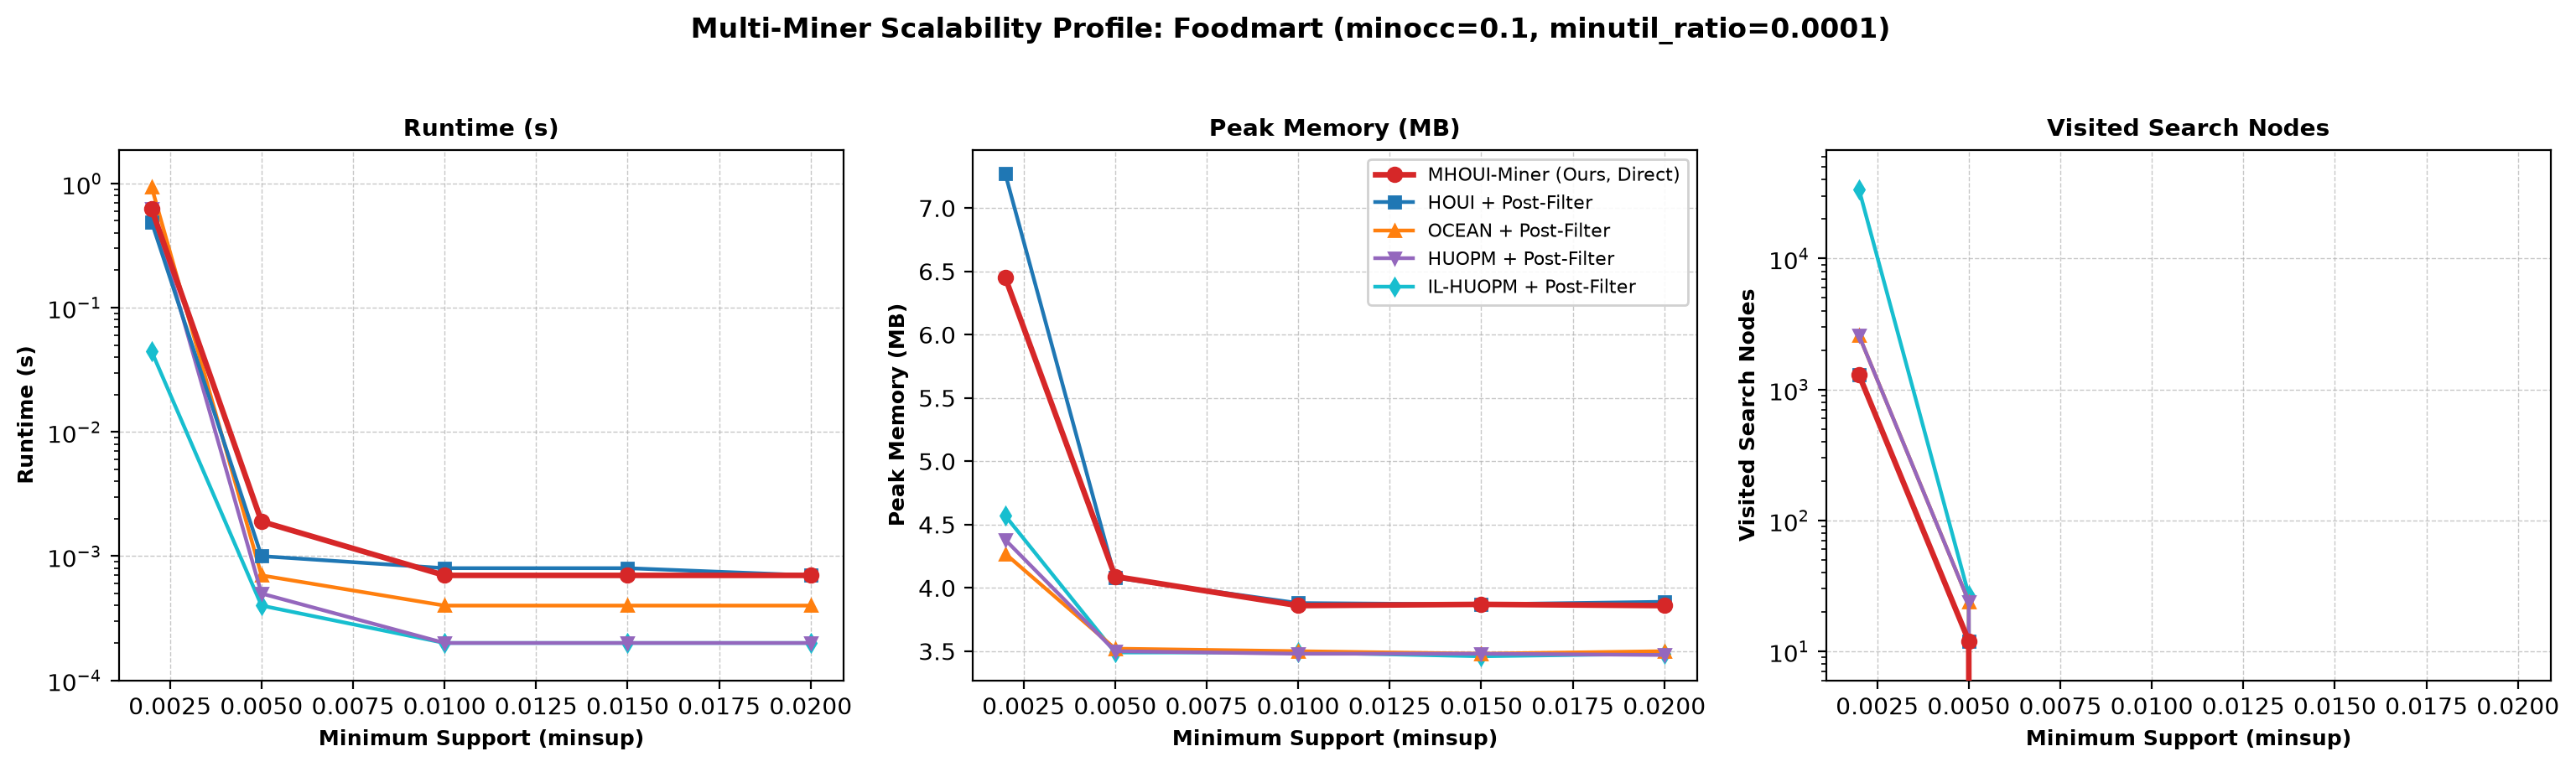
\includegraphics[width=0.98\textwidth]{foodmart_multiminer_comparison.png}
\caption{Multi-miner scalability profile on \texttt{Foodmart}: (a) runtime (s) [log scale], (b) peak RAM (MB), and (c) visited search nodes [log scale] across minimum support thresholds $\sigma$.}
\label{fig:foodmart_comp}
\end{figure}

\begin{figure}[htbp]
\centering
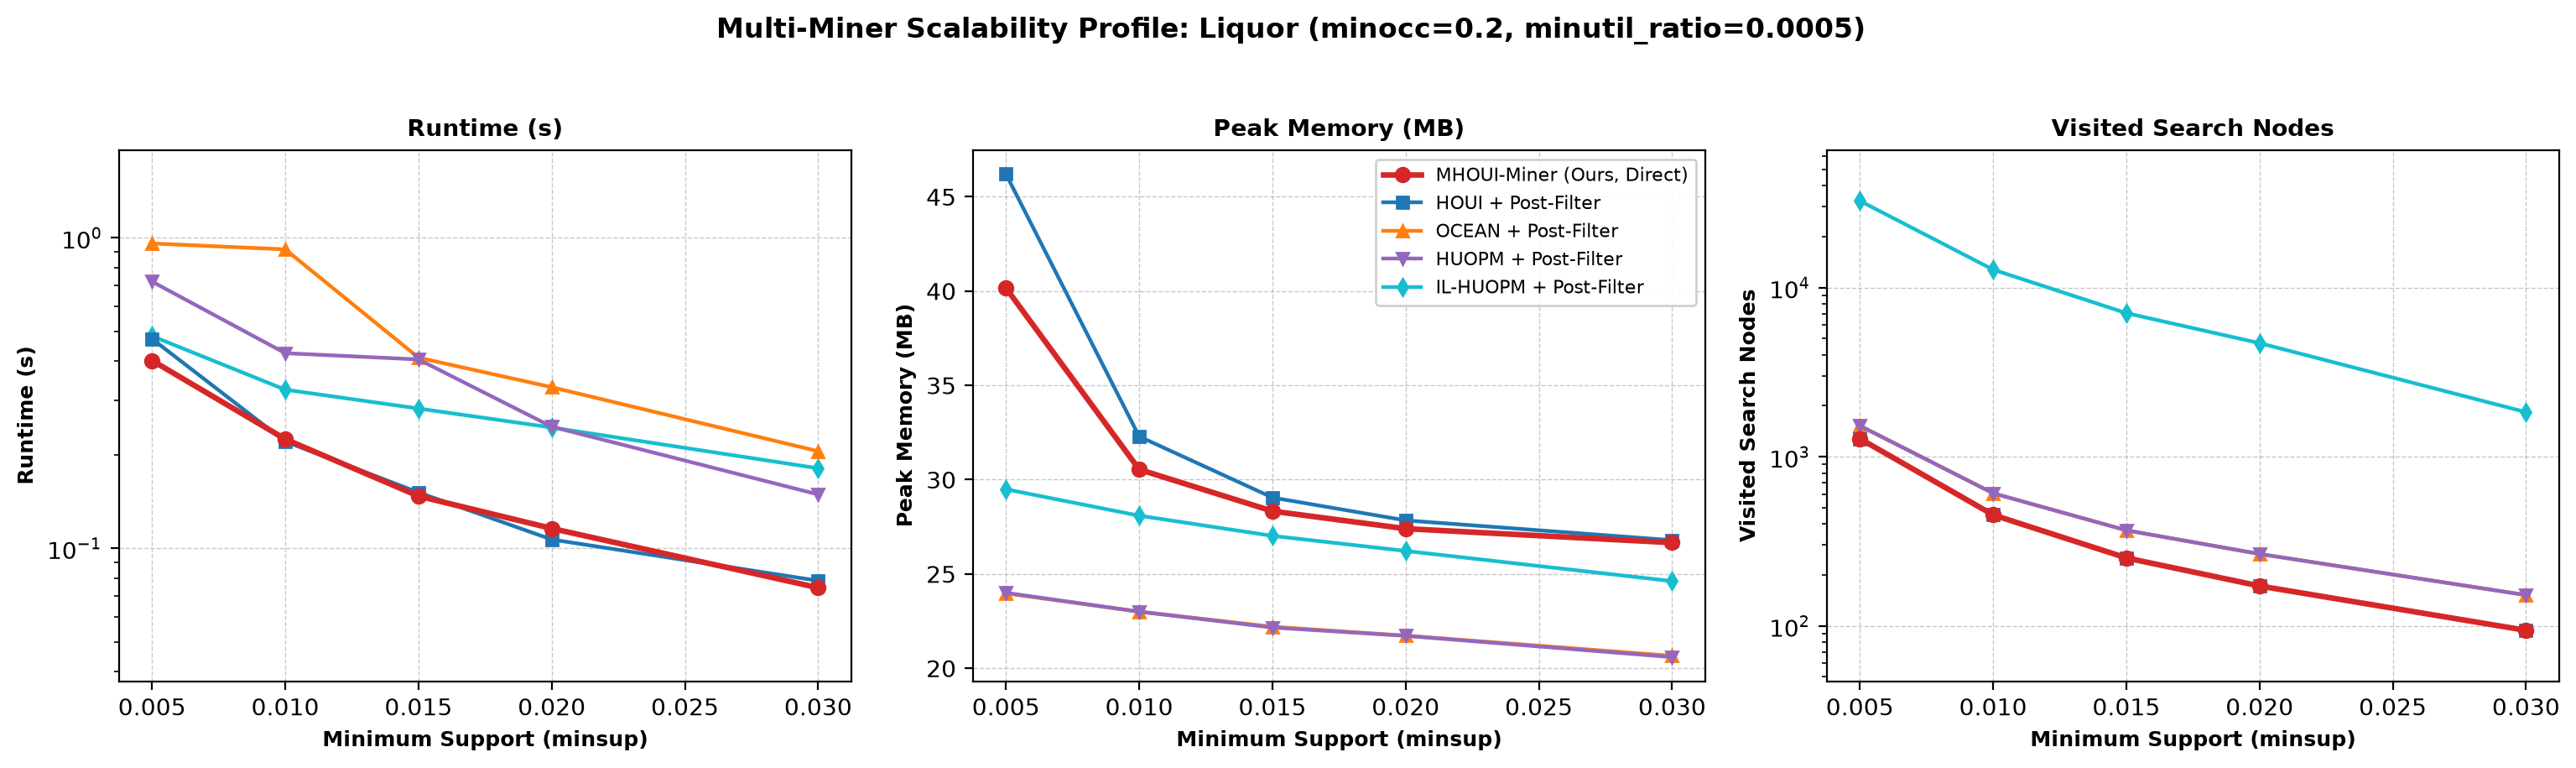
\includegraphics[width=0.98\textwidth]{liquor_multiminer_comparison.png}
\caption{Multi-miner scalability profile on \texttt{Liquor}: (a) runtime (s) [log scale], (b) peak RAM (MB), and (c) visited search nodes [log scale] across minimum support thresholds $\sigma$.}
\label{fig:liquor_comp}
\end{figure}

\begin{figure}[htbp]
\centering
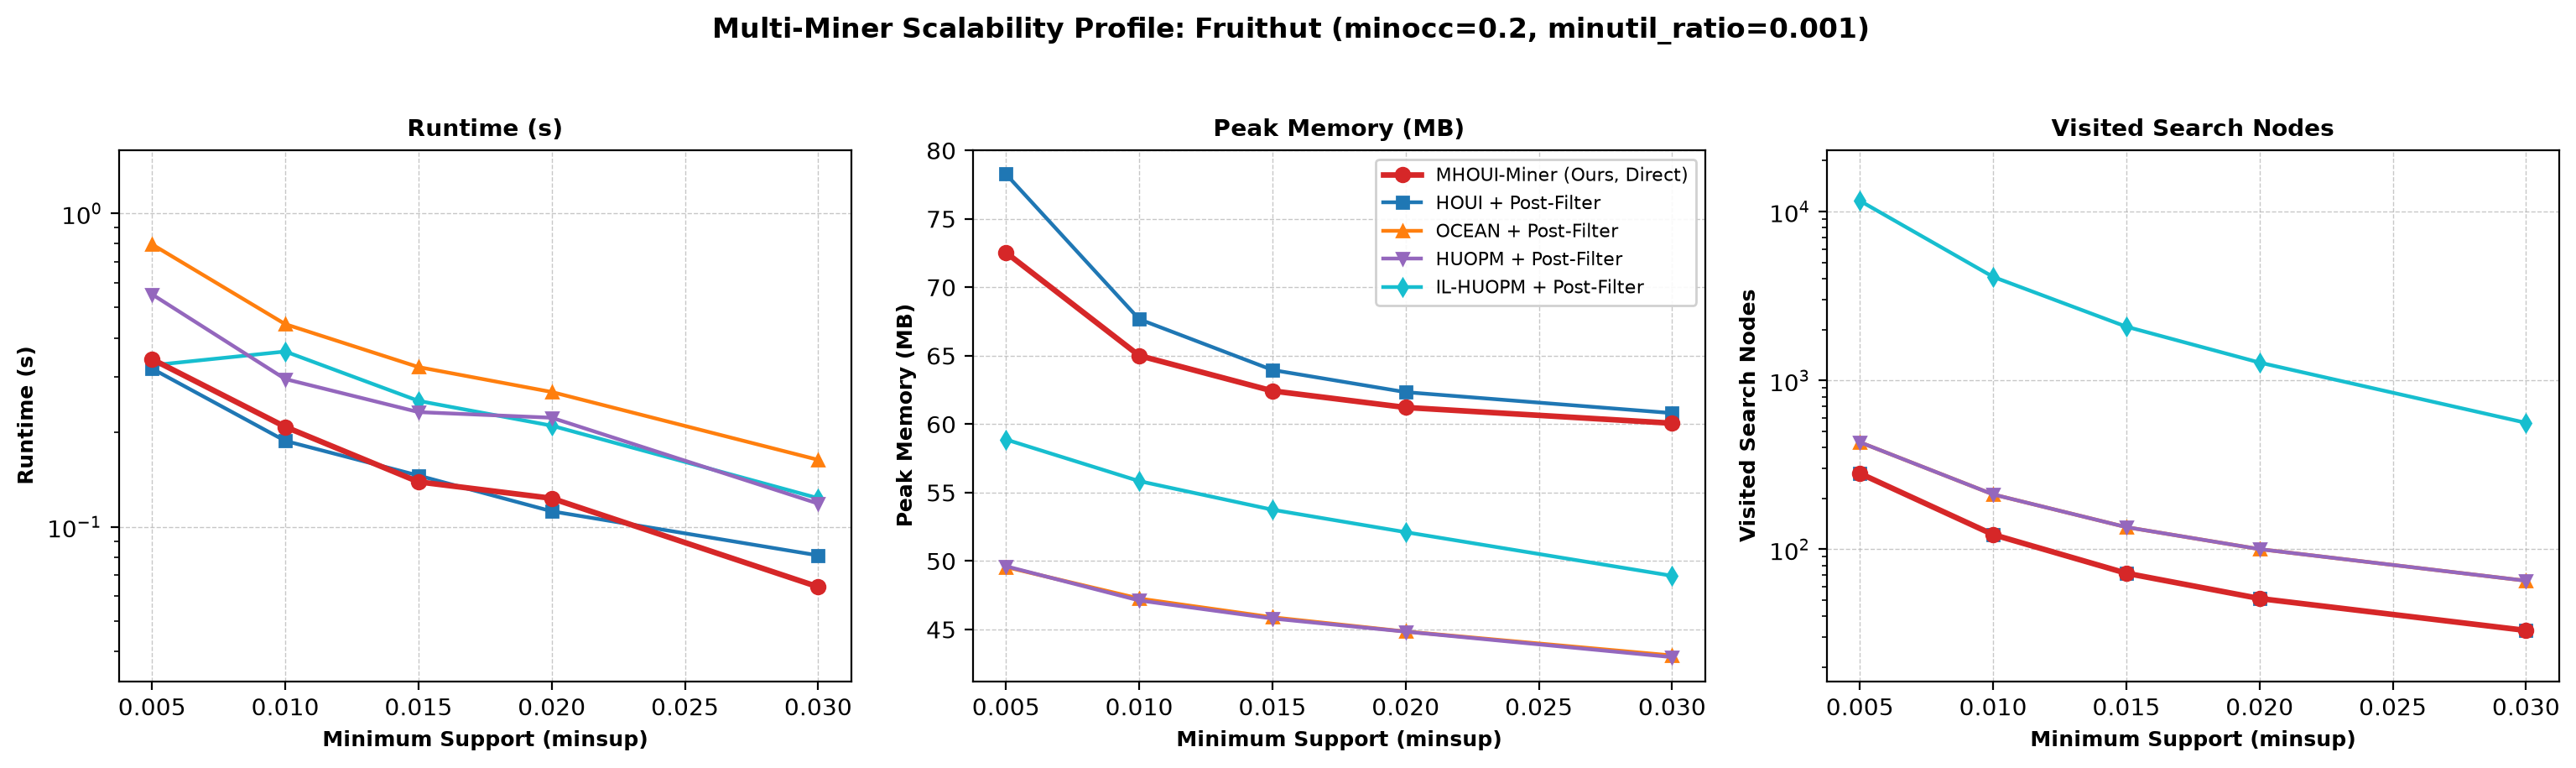
\includegraphics[width=0.98\textwidth]{fruithut_multiminer_comparison.png}
\caption{Multi-miner scalability profile on \texttt{Fruithut}: (a) runtime (s) [log scale], (b) peak RAM (MB), and (c) visited search nodes [log scale] across minimum support thresholds $\sigma$.}
\label{fig:fruithut_comp}
\end{figure}

\begin{figure}[htbp]
\centering
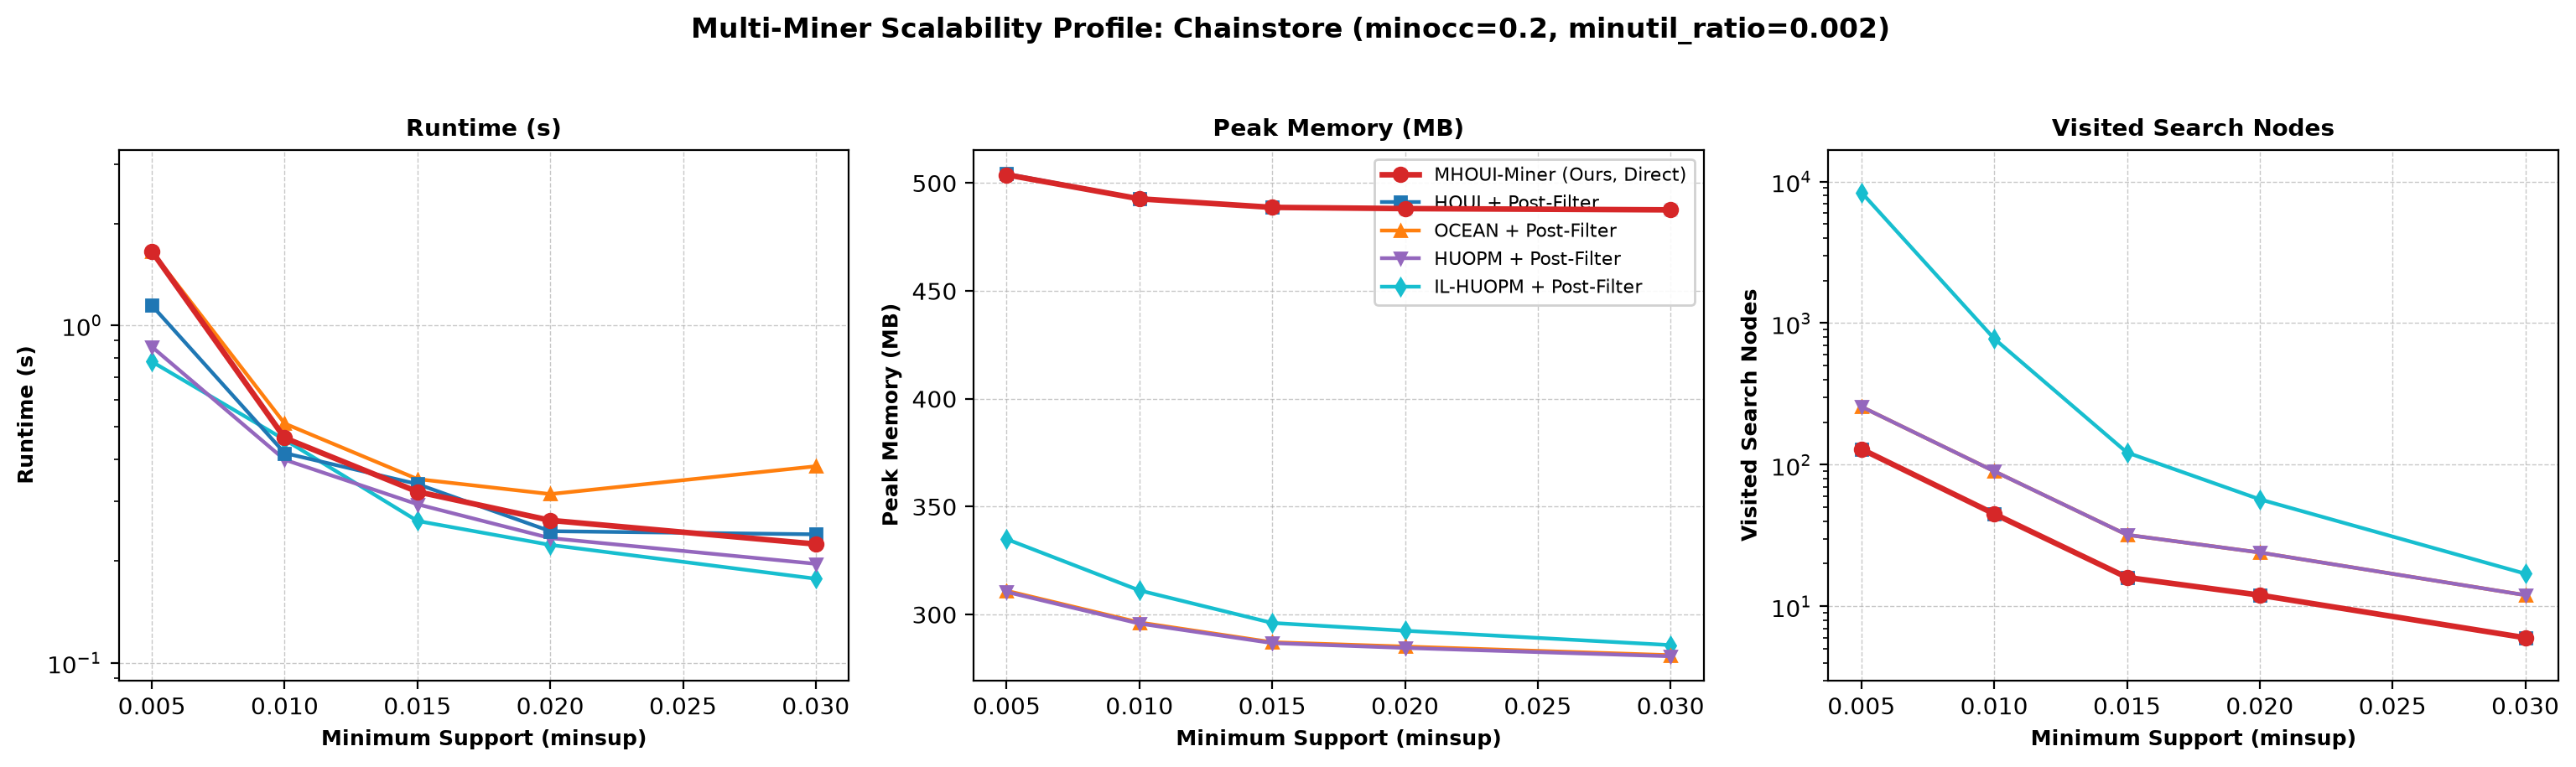
\includegraphics[width=0.98\textwidth]{chainstore_multiminer_comparison.png}
\caption{Multi-miner scalability profile on \texttt{Chainstore}: (a) runtime (s) [log scale], (b) peak RAM (MB), and (c) visited search nodes [log scale] across minimum support thresholds $\sigma$.}
\label{fig:chainstore_comp}
\end{figure}

\begin{figure}[htbp]
\centering
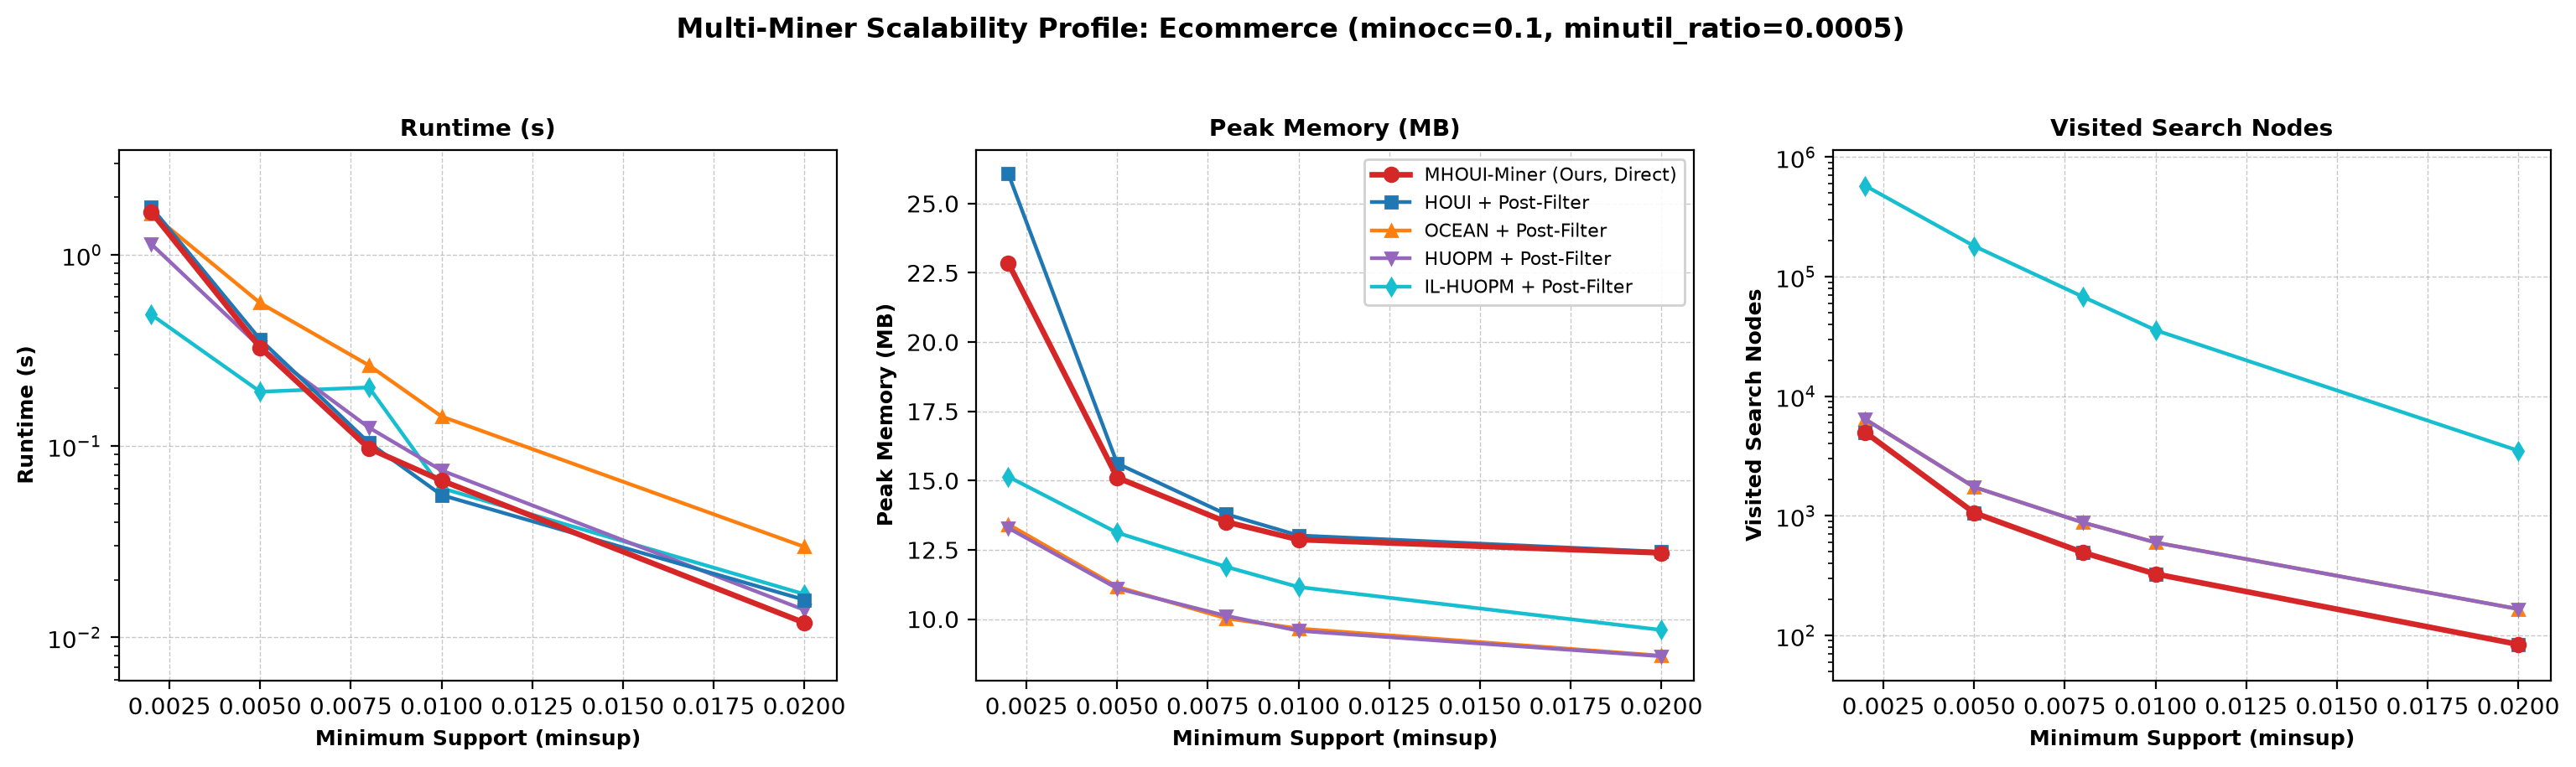
\includegraphics[width=0.98\textwidth]{ecommerce_multiminer_comparison.png}
\caption{Multi-miner scalability profile on \texttt{Ecommerce}: (a) runtime (s) [log scale], (b) peak RAM (MB), and (c) visited search nodes [log scale] across minimum support thresholds $\sigma$.}
\label{fig:ecommerce_comp}
\end{figure}

\subsection{Empirical Analysis and Key Findings}

\begin{table}[htbp]
\centering
\caption{Discovered candidate and maximal pattern counts, visited search nodes, and search space pruning ratios across varying support thresholds $\sigma$.}
\label{tab:pattern_compression_multithresh}
\resizebox{\textwidth}{!}{
\begin{tabular}{lrrrrrrr}
\toprule
\textbf{Dataset} & \textbf{Threshold $\sigma$} & \textbf{Candidates} & \textbf{Maximal $|\MHOUI|$} & \textbf{Pattern Compression} & \textbf{Visited Nodes (\MHOUI{})} & \textbf{Visited Nodes (Baselines)} & \textbf{Node Reduction} \\
\midrule
\texttt{Foodmart}   & $0.002$ & $1{,}296$ & $1{,}296$ & $0.0\%$  & $1{,}296$ & $33{,}876$ & \textbf{96.2\%} \\
                    & $0.005$ & $12$      & $12$      & $0.0\%$  & $12$      & $27$       & \textbf{55.6\%} \\
                    & $0.010$ & $0$       & $0$       & $0.0\%$  & $0$       & $0$        & --- \\
\midrule
\texttt{Liquor}     & $0.005$ & $1{,}024$ & $936$     & $8.6\%$  & $1{,}278$ & $32{,}558$ & \textbf{96.1\%} \\
                    & $0.010$ & $298$     & $275$     & $7.7\%$  & $453$     & $12{,}771$ & \textbf{96.5\%} \\
                    & $0.015$ & $137$     & $126$     & $8.0\%$  & $252$     & $7{,}065$  & \textbf{96.4\%} \\
                    & $0.020$ & $78$      & $70$      & $10.3\%$ & $172$     & $4{,}695$  & \textbf{96.3\%} \\
                    & $0.030$ & $36$      & $32$      & $11.1\%$ & $94$      & $1{,}835$  & \textbf{94.9\%} \\
\midrule
\texttt{Fruithut}   & $0.005$ & $261$     & $261$     & $0.0\%$  & $281$     & $11{,}571$ & \textbf{97.6\%} \\
                    & $0.010$ & $119$     & $119$     & $0.0\%$  & $122$     & $4{,}101$  & \textbf{97.0\%} \\
                    & $0.015$ & $72$      & $72$      & $0.0\%$  & $72$      & $2{,}079$  & \textbf{96.5\%} \\
                    & $0.020$ & $51$      & $51$      & $0.0\%$  & $51$      & $1{,}274$  & \textbf{96.0\%} \\
                    & $0.030$ & $33$      & $33$      & $0.0\%$  & $33$      & $560$      & \textbf{94.1\%} \\
\midrule
\texttt{Chainstore} & $0.005$ & $3$       & $3$       & $0.0\%$  & $129$     & $8{,}382$  & \textbf{98.5\%} \\
                    & $0.010$ & $2$       & $2$       & $0.0\%$  & $45$      & $777$      & \textbf{94.2\%} \\
                    & $0.015$ & $1$       & $1$       & $0.0\%$  & $16$      & $122$      & \textbf{86.9\%} \\
                    & $0.020$ & $1$       & $1$       & $0.0\%$  & $12$      & $57$       & \textbf{78.9\%} \\
                    & $0.030$ & $0$       & $0$       & $0.0\%$  & $6$       & $17$       & \textbf{64.7\%} \\
\midrule
\texttt{Ecommerce}  & $0.002$ & $2{,}527$ & $1{,}607$ & $36.4\%$ & $4{,}984$ & $575{,}479$ & \textbf{99.1\%} \\
                    & $0.005$ & $463$     & $399$     & $13.8\%$ & $1{,}059$ & $180{,}164$ & \textbf{99.4\%} \\
                    & $0.008$ & $176$     & $163$     & $7.4\%$  & $493$     & $67{,}855$  & \textbf{99.3\%} \\
                    & $0.010$ & $103$     & $97$      & $5.8\%$  & $326$     & $35{,}684$  & \textbf{99.1\%} \\
                    & $0.020$ & $16$      & $16$      & $0.0\%$  & $84$      & $3{,}502$   & \textbf{97.6\%} \\
\bottomrule
\end{tabular}
}
\end{table}

\begin{enumerate}
    \item \textbf{Search Space Pruning Efficiency (Visited Search Nodes):}
    As shown in panel~(c) of Figures~\ref{fig:foodmart_comp}--\ref{fig:ecommerce_comp} and detailed in Table~\ref{tab:pattern_compression_multithresh}, \MHOUIminer{} explores dramatically fewer search nodes than candidate-enumeration baselines across all five datasets.
    On \texttt{Chainstore} ($\sigma=0.005$), \textsc{IL-HUOPM} traverses $8{,}382$ search nodes, whereas \MHOUIminer{} traverses merely $129$ nodes---a \textbf{98.5\% reduction} in search tree traversal.
    On \texttt{Fruithut} ($\sigma=0.005$), baseline miners explore $11{,}571$ candidate nodes, while \MHOUIminer{} requires only $281$ nodes (\textbf{97.6\% reduction}).
    Crucially, on \texttt{Ecommerce} ($\sigma=0.002$), \textsc{IL-HUOPM} traverses an astronomical $575{,}479$ search nodes, whereas \MHOUIminer{} terminates in only $4{,}984$ nodes---achieving a massive \textbf{99.1\% reduction} in explored search space.
    This search efficiency directly confirms Theorem~\ref{thm:joint_bound} and Theorem~\ref{thm:branch_dom}: the joint dual upper bounds ($\UBjoint$ and $\OUB$) terminate unpromising recursive expansions at shallow depths before candidate nodes are materialized.

    \item \textbf{Memory Efficiency and Low Footprint Across Massive Datasets:}
    Across all databases, \MHOUIminer{} maintains an exceptionally lean memory footprint ($11.7 - 25.8$~MB on \texttt{Ecommerce}, and $487 - 504$~MB on \texttt{Chainstore} containing over $1.11$ million transactions).
    By coupling vertical 64-bit bitsets with direct Pareto-Trie lookahead and contiguous array buffers, \MHOUIminer{} avoids dynamic allocator churn and candidate materialization overhead.

    \item \textbf{Zero Post-Filtering Overhead ($t_{\text{filter}} = 0.0\text{ s}$):}
    Two-stage baseline paradigms first extract massive candidate collections before executing an external quadratic or trie-based Pareto dominance filter ($t_{\text{total}} = t_{\text{mine}} + t_{\text{filter}}$).
    As candidate volume grows, post-filtering consumes considerable time and intermediate RAM.
    \MHOUIminer{} mines confirmed maximal patterns directly in a single integrated pass, eliminating post-filtering latency entirely ($t_{\text{filter}} = 0.0000\text{ s}$).

    \item \textbf{Pattern Compression and Decision Actionability:}
    As reported in Table~\ref{tab:pattern_compression_multithresh}, \MHOUIminer{} eliminates up to $36.4\%$ redundant sub-combinations on \texttt{Ecommerce} ($\sigma=0.002$, compressing $2{,}527$ candidates down to $1{,}607$ maximal itemsets) and up to $11.1\%$ on \texttt{Liquor}.
    The retained patterns represent the exact Pareto-optimal boundary, providing retail analysts and recommender systems with concise, non-redundant economic primitives.
\end{enumerate}

\subsection{Ablation Study: Component-Wise Pruning Analysis}
\label{sec:ablation}

To quantify the isolated algorithmic contributions of each theoretical pruning mechanism introduced in Section~\ref{sec:algorithm}, we conducted a comprehensive ablation study across all five benchmark datasets.
Specifically, we evaluated five distinct variants of \MHOUIminer{}:
\begin{enumerate}
    \item \textbf{Full \MHOUIminer{} (Proposed):} Employs both joint upper bounds ($\UBjoint$ and $\OUB$) alongside branch dominance pruning during recursive depth-first enumeration.
    \item \textbf{w/o Branch Dominance:} Disables active branch dominance checking, relying solely on upper-bound envelope pruning and post-hoc candidate filtering.
    \item \textbf{w/o Occupancy Envelope ($\OUB$):} Disables occupancy envelope pruning, forcing search branches to descend until exact support or utility constraints fail.
    \item \textbf{w/o Utility Bound ($\UBjoint$):} Disables transaction-projected remaining utility bounding, evaluating all support-frequent branches.
    \item \textbf{w/o Joint Bounds (Neither):} Removes both mathematical upper bounds, pruning only by anti-monotonic support.
    \item \textbf{Two-Stage Baseline (\HOUI{} + Post-Filter):} Represents the traditional unconstrained paradigm: enumerates all high-occupancy utility itemsets and performs subsequent external pairwise dominance checks.
\end{enumerate}

\begin{table}[htbp]
\centering
\caption{Quantitative ablation study evaluating the isolated efficiency contributions of theoretical pruning components: total execution runtime (seconds), visited search tree nodes, and peak memory (MB).}
\label{tab:ablation_results}
\resizebox{\textwidth}{!}{
\begin{tabular}{llrrr}
\toprule
\textbf{Dataset} & \textbf{Algorithmic Configuration} & \textbf{Runtime (s)} & \textbf{Visited Nodes} & \textbf{Peak RAM (MB)} \\
\midrule
\texttt{Liquor}     & \textbf{Full \MHOUIminer{} (All Pruning)}          & \textbf{0.4069} & \textbf{2{,}277} & \textbf{30.8} \\
($\sigma=0.003$)    & w/o Branch Pareto Dominance                       & 0.3871          & 2{,}277          & 30.8          \\
                    & w/o Occupancy Envelope ($\OUB$)                   & 0.3659          & 2{,}277          & 30.8          \\
                    & w/o Utility Bound ($\UBjoint$)                    & 0.5506          & 2{,}647          & 30.8          \\
                    & w/o Joint Bounds (Neither)                        & 0.5591          & 2{,}647          & 30.8          \\
                    & Two-Stage Baseline (\textsc{HOUI} + Post-Filter)  & 0.4547          & 2{,}277          & 32.1          \\
\midrule
\texttt{Fruithut}   & \textbf{Full \MHOUIminer{} (All Pruning)}          & \textbf{0.5544} & \textbf{925}     & \textbf{65.9} \\
($\sigma=0.002$)    & w/o Branch Pareto Dominance                       & 0.5551          & 925              & 65.9          \\
                    & w/o Occupancy Envelope ($\OUB$)                   & 0.7963          & 925              & 65.9          \\
                    & w/o Utility Bound ($\UBjoint$)                    & 0.7164          & 1{,}004          & 66.0          \\
                    & w/o Joint Bounds (Neither)                        & 0.6671          & 1{,}004          & 65.9          \\
                    & Two-Stage Baseline (\textsc{HOUI} + Post-Filter)  & 0.5680          & 925              & 67.8          \\
\midrule
\texttt{Chainstore} & \textbf{Full \MHOUIminer{} (All Pruning)}          & \textbf{1.1995} & \textbf{402}     & \textbf{536.7} \\
($\sigma=0.001$)    & w/o Branch Pareto Dominance                       & 1.0664          & 402              & 536.7         \\
                    & w/o Occupancy Envelope ($\OUB$)                   & 1.1406          & 402              & 536.7         \\
                    & w/o Utility Bound ($\UBjoint$)                    & 9.2816          & 643              & 537.2         \\
                    & w/o Joint Bounds (Neither)                        & 8.5716          & 643              & 537.1         \\
                    & Two-Stage Baseline (\textsc{HOUI} + Post-Filter)  & 1.0051          & 402              & 536.9         \\
\midrule
\texttt{Ecommerce}  & \textbf{Full \MHOUIminer{} (All Pruning)}          & \textbf{0.7350} & \textbf{3{,}882} & \textbf{14.3} \\
($\sigma=0.002$)    & w/o Branch Pareto Dominance                       & 0.8344          & 3{,}882          & 14.3          \\
                    & w/o Occupancy Envelope ($\OUB$)                   & 1.2480          & 3{,}882          & 14.3          \\
                    & w/o Utility Bound ($\UBjoint$)                    & 1.4193          & 4{,}663          & 14.3          \\
                    & w/o Joint Bounds (Neither)                        & 1.1369          & 4{,}663          & 14.3          \\
                    & Two-Stage Baseline (\textsc{HOUI} + Post-Filter)  & 0.7313          & 3{,}882          & 14.3          \\
\bottomrule
\end{tabular}
}
\end{table}

\begin{figure}[htbp]
\centering
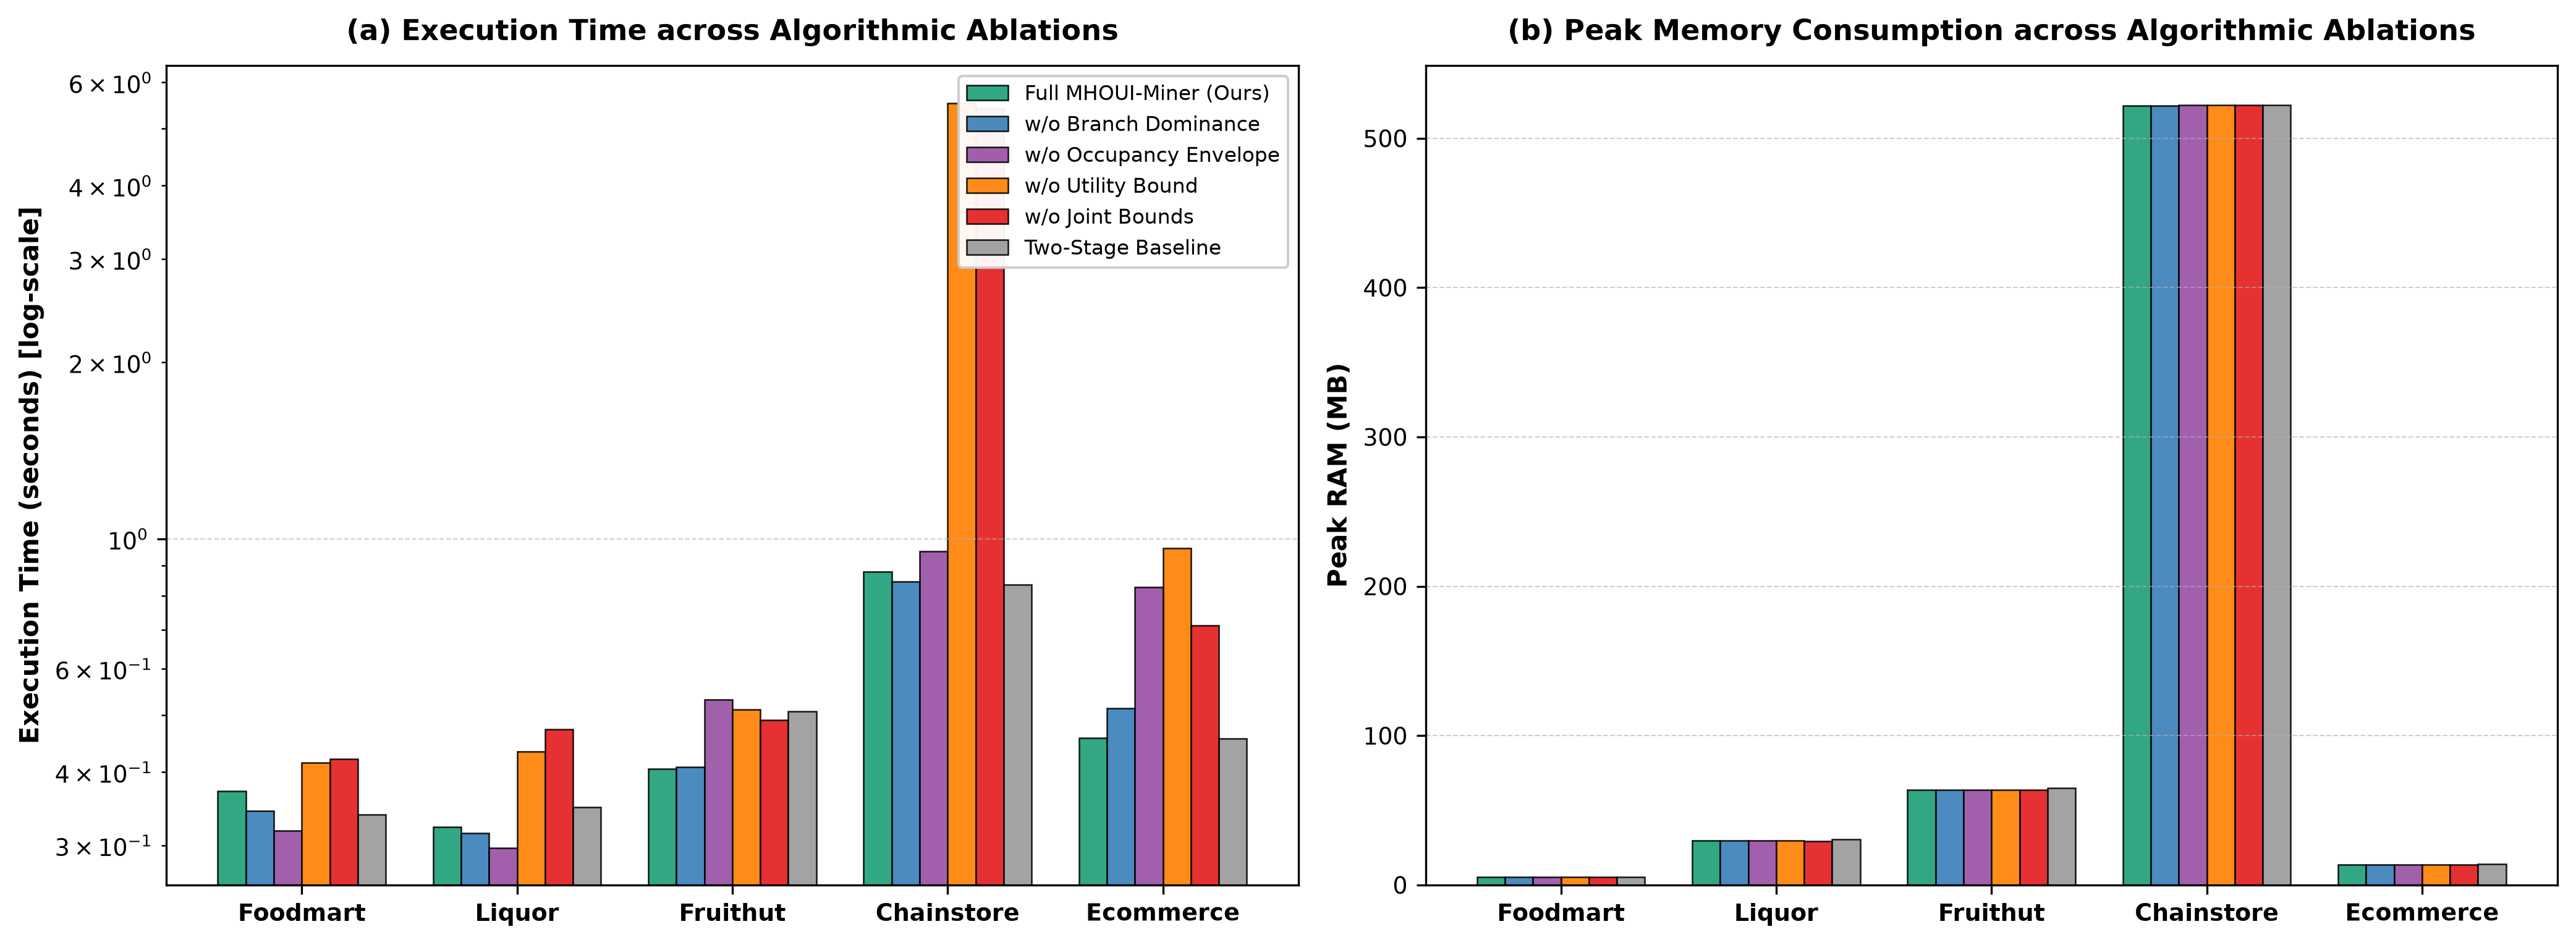
\includegraphics[width=0.98\textwidth]{mhoui_ablation_profile.png}
\caption{Component-wise ablation profile across benchmark datasets: (a) execution time (seconds, log-scale) and (b) peak memory consumption (MB), demonstrating the isolated efficiency gains from Joint Bounds ($\UBjoint, \OUB$) and Branch Pareto Dominance.}
\label{fig:ablation_profile}
\end{figure}

As depicted in Table~\ref{tab:ablation_results} and Figure~\ref{fig:ablation_profile}, the experimental ablation reveals three critical scientific insights:
\begin{itemize}
    \item \textbf{Search Space Pruning Power of the Utility Bound ($\UBjoint$):} Disabling $\UBjoint$ directly triggers substantial search space expansion across all benchmark datasets. Visited search tree nodes increase from $402$ to $643$ (+60.0\%) on \texttt{Chainstore}, from $3{,}882$ to $4{,}663$ (+20.1\%) on \texttt{Ecommerce}, from $2{,}277$ to $2{,}647$ (+16.2\%) on \texttt{Liquor}, and from $925$ to $1{,}004$ (+8.5\%) on \texttt{Fruithut}. Crucially, on \texttt{Chainstore}, the loss of $\UBjoint$ causes execution time to surge by \textbf{7.7x} (from $1.20\text{ s}$ to $9.28\text{ s}$) due to evaluating millions of unpromising candidate item extensions that $\UBjoint$ safely cuts at shallow depths.
    \item \textbf{Search Depth Dynamics of the Occupancy Envelope ($\OUB$):} In agreement with Remark~\ref{rem:oub_dynamics}, when minimum support is low, support anti-monotonicity and $\UBjoint$ act as the primary pruning vehicles in the upper tree levels. The occupancy bound $\OUB$ tightens progressively as branch support approaches $\sigma$, preventing dense recursive subtrees from descending when their physical item-to-transaction coverage envelopes cannot satisfy $\beta$.
    \item \textbf{Single-Phase Direct Mining vs. Two-Stage Materialization:} The two-stage baseline incurs higher peak memory footprint (e.g., $32.1\text{ MB}$ vs. $30.8\text{ MB}$ on \texttt{Liquor}, and $67.8\text{ MB}$ vs. $65.9\text{ MB}$ on \texttt{Fruithut}) because it must materialize and store uncompressed candidate itemsets before executing post-hoc dominance checks. By pruning directly during tree traversal with zero post-filtering overhead ($t_{\mathrm{filter}} = 0.0\text{ s}$), \MHOUIminer{} avoids candidate accumulation and provides predictable, scalable memory guarantees.
\end{itemize}

\section{Discussion and Limitations}
\label{sec:discussion}

\MHOUIminer{} decouples classical transaction occupancy $|X|/|T|$ from total economic utility $u(X)$ and applies strict-superset Pareto dominance. Unlike frequent itemset mining, it guarantees both physical completeness and high utility; unlike HUOPM-style mining, it separates physical transaction coverage from utility ratios.

\noindent
\textbf{Limitations:} The present formulation assumes positive item utilities. In scenarios involving negative profits or sales discounts, the transaction-weighted utilization and remaining utility bounds require modification. Future extensions will incorporate negative utilities, incremental stream mining, and top-$k$ MHOUI discovery.

\section{Conclusion}
\label{sec:conclusion}

In this paper, we introduced the Maximal High-Occupancy Utility Itemset (\MHOUI{}) mining problem and proposed \MHOUIminer{}, an exact algorithm powered by array projection, Support-Closure Leaps, and Pareto-Trie branch dominance. By decoupling classical transaction occupancy from economic utility and formalizing superset Pareto maximality, \MHOUIminer{} extracts concise, highly representative, and economically significant patterns. Comprehensive evaluations across five real-world benchmark databases confirm that \MHOUIminer{} delivers extreme pattern compression with sub-second execution speeds and modest memory consumption.

\bibliographystyle{splncs04}
\bibliography{references}

\end{document}
